\documentclass[]{afit-etd}

% The afit-etd class requires the following packages: url, refcount, graphicx,
%                                                     sf298, hyperref

% The following packages and macros are recommended but not required:
\usepackage{xcolor}                  % standard package for including colors
\usepackage[square,sort&compress,numbers]{natbib} % better citations
                                % especially when including a string of
                                % citations
%\newcommand\citenum[1]{#1}

% Packages for fonts
\usepackage{amssymb}  % math symbols (amsmath & amsthm are defined in afit-etd)
\usepackage[printonlyused,withpage]{acronym}
\usepackage{lettrine} % provides dropped characters to lead off a paragraph.
                      % These are not required, but some people like them at
                      % the start of each chapter.
\usepackage{bm}       % The most comprehensive package for bold math figures
\usepackage{textcomp} % \texttimes, \textdegree, \textohm, \textmu

% Packages for tables
\usepackage{booktabs} % improved rules (lines) for tables
\usepackage{dcolumn}  % align at decimal in tables
\usepackage{multirow} % table elements spanning multiple rows

\graphicspath{{diagrams/}} % reduce clutter by storing figures elsewhere

% Other stuff I want
\usepackage{graphicx, color}
%% maxwidth is the original width if it is less than linewidth
%% otherwise use linewidth (to make sure the graphics do not exceed the margin)
\makeatletter
\def\maxwidth{ %
  \ifdim\Gin@nat@width>\linewidth
    \linewidth
  \else
    \Gin@nat@width
  \fi
}
\makeatother

\IfFileExists{upquote.sty}{\usepackage{upquote}}{}
\definecolor{fgcolor}{rgb}{0.2, 0.2, 0.2}
\newcommand{\hlnumber}[1]{\textcolor[rgb]{0,0,0}{#1}}%
\newcommand{\hlfunctioncall}[1]{\textcolor[rgb]{0.501960784313725,0,0.329411764705882}{\textbf{#1}}}%
\newcommand{\hlstring}[1]{\textcolor[rgb]{0.6,0.6,1}{#1}}%
\newcommand{\hlkeyword}[1]{\textcolor[rgb]{0,0,0}{\textbf{#1}}}%
\newcommand{\hlargument}[1]{\textcolor[rgb]{0.690196078431373,0.250980392156863,0.0196078431372549}{#1}}%
\newcommand{\hlcomment}[1]{\textcolor[rgb]{0.180392156862745,0.6,0.341176470588235}{#1}}%
\newcommand{\hlroxygencomment}[1]{\textcolor[rgb]{0.43921568627451,0.47843137254902,0.701960784313725}{#1}}%
\newcommand{\hlformalargs}[1]{\textcolor[rgb]{0.690196078431373,0.250980392156863,0.0196078431372549}{#1}}%
\newcommand{\hleqformalargs}[1]{\textcolor[rgb]{0.690196078431373,0.250980392156863,0.0196078431372549}{#1}}%
\newcommand{\hlassignement}[1]{\textcolor[rgb]{0,0,0}{\textbf{#1}}}%
\newcommand{\hlpackage}[1]{\textcolor[rgb]{0.588235294117647,0.709803921568627,0.145098039215686}{#1}}%
\newcommand{\hlslot}[1]{\textit{#1}}%
\newcommand{\hlsymbol}[1]{\textcolor[rgb]{0,0,0}{#1}}%
\newcommand{\hlprompt}[1]{\textcolor[rgb]{0.2,0.2,0.2}{#1}}%

\usepackage{framed}
\makeatletter
\newenvironment{kframe}{%
 \def\at@end@of@kframe{}%
 \ifinner\ifhmode%
  \def\at@end@of@kframe{\end{minipage}}%
  \begin{minipage}{\columnwidth}%
 \fi\fi%
 \def\FrameCommand##1{\hskip\@totalleftmargin \hskip-\fboxsep
 \colorbox{shadecolor}{##1}\hskip-\fboxsep
     % There is no \\@totalrightmargin, so:
     \hskip-\linewidth \hskip-\@totalleftmargin \hskip\columnwidth}%
 \MakeFramed {\advance\hsize-\width
   \@totalleftmargin\z@ \linewidth\hsize
   \@setminipage}}%
 {\par\unskip\endMakeFramed%
 \at@end@of@kframe}
\makeatother

\definecolor{shadecolor}{rgb}{.97, .97, .97}
\definecolor{messagecolor}{rgb}{0, 0, 0}
\definecolor{warningcolor}{rgb}{1, 0, 1}
\definecolor{errorcolor}{rgb}{1, 0, 0}
\newenvironment{knitrout}{}{} % an empty environment to be redefined in TeX

\usepackage{alltt}

 
\usepackage[section]{placeins}
\usepackage{comment}
\usepackage{listings}
\usepackage{enumerate}
\usepackage{caption}
\usepackage{subcaption}
\usepackage{colortbl}

\usepackage{float}
 
\floatstyle{plaintop}
\restylefloat{table}
\floatstyle{plain}
\restylefloat{figure}

\usepackage{pdflscape}

% Warning! This must be included after everything else! The afit-cls class attempts to
% include this, but it's far too early
\usepackage[bookmarks, breaklinks, colorlinks, linkcolor=black, urlcolor=black, citecolor=black]{hyperref}

\lstloadlanguages{Python, C, bash}
\lstset{
	numberbychapter=true,
	captionpos=t,
	language=bash,
	tabsize=4,
	breaklines=true,
	breakatwhitespace=true,
	prebreak=\textbackslash,
	basicstyle=\small\ttfamily,
	xleftmargin=10pt,
	xrightmargin=10pt,
	framesep=5pt,
	framerule=2pt,
	frame=leftline,
	rulecolor=\color{gray},
	numbers=left,
    numberstyle=\small\color{black!85},
    stepnumber=1, 
    numbersep=13pt,
    backgroundcolor=\color{black!5},
}

% Command line/terminal-like environment
% Todo tag
\newcommand{\tbd}[1]{{\color{red} TBD: #1}}



%%%%% Required front matter definitions %%%%%%%%%%%%%%%%%%%%%%%%%%%%%%%%%%%%%%%

\title  {Malicious Traffic Detection through Internet Protocol Address Hopping}
\doctype{THESIS} % or GRADUATE RESEARCH PAPER, DISSERTATION, or REPORT
                 % REPORT will generate a simplified format more suitable for
                 % class assignments

\author          {Ryan A.}{Morehart}
\rank            {Second Lieutenant, USAF}
\previousdegrees {B.S.} % Abbreviate any previous degrees

% Uncomment the following lines if there is a second author
% \coauthor          {FirstName I. LastName} 
% \corank            {Major, USAF}
% \copreviousdegrees {B.S.} 

\degree          {Master of Science}
\graduation      {27}{March}{2013} % format is {DD}{Month}{YYYY} where
                                   % Month must be: March, June,
                                   % September, or December

\designator{AFIT-ENG-13-M-35}

\distribution{DISTRIBUTION STATEMENT A:\\APPROVED FOR PUBLIC RELEASE;
  DISTRIBUTION UNLIMITED} % or other appropriate distribution statement from the
                          % AFIT Style Guide

\committee{ % Advisor must be listed first in the list of committee members
  {Dr. Barry Mullins, PhD (Chairman)},
  {Dr. Rusty Baldwin, PhD (Member)},
  {Dr. Timothy Lacey, PhD (Member)}
}

\department {Department of Electrical and Computer Engineering}
%\deptsymbol {ENG}

\school     {Graduate School of Engineering and Management}
\dean       {M. U. Thomas} % only used for PhD dissertations

% Uncomment the following line to switch from blank signature lines on
% the approval page to lines marked with ``/signed/'' and the
% corresponding dates.  This avoid having to scan the signature page into the
% final PDF document for the electronic version, but it also doesn't look as 
% professional.  Similarly, the Dean's signature can be indicated using the 
% second line below.  Note that the original signatures are still required on
% the hardcopy submitted to the library.

% \committeeSignedDates{2 Jun 2011,3 Jun 2011,4 Jun 2011}
% \deanSignedDate{9 Jun 2011}

\abstract{\par This thesis explores the viability of using \ac{IP} address hopping in front of a network as a defensive measure. Network address space randomization techniques theoretically provide protection to a network by appearing to randomly change the addresses of hosts inside, presenting a challenge to an intruder attempting to break in and map the network. This research presents a custom gateway-based \ac{IP} hopping solution called \ac{ARG} that combines previous work in this area.

\par \ac{ARG} works as a transparent gateway in front of a network, requiring no changes to the hosts inside or out. Each \ac{ARG} gateway is configured with a small amount of knowledge on one or more other gateways, allowing them to connect and pass fully encrypted and authenticated traffic amongst themselves. Connections to non-\ac{ARG} networks or hosts are handled gracefully, allowing long-lived connections to exist without terminating them during \ac{IP} address changes. This thesis tests the overall stability of \ac{ARG}, the accuracy of its classifications, the maximum throughput it can support, and the maximum rate at which it can change \acp{IP} and still communication reliably.

\par This research is done on a physical test network with nodes representing the types of hosts found on a typical, corporate-style network. Measurement is used to obtain all results for each factor level. Tests demonstrate \ac{ARG} classifies traffic correctly, with no false negatives and less than a 0.15\% false positive rate on average. This remains true as long as the time between \ac{IP} address changes exceeds four times the one-way latency on the network, although test conditions give reason to suspect the hop rate could be closer to the latency in real operation. Results show \ac{ARG} capably handles traffic of at least four megabits per second with no impact on packet loss. Fuzz testing validates the stability of \ac{ARG} itself, although additional packet loss of around 23\% appears when under attack.

\acresetall

}

%%%% Required SF298 macros %%%%%%%%%%%%%%%%%%%%%%%%%%%%%%%%%%%%%%%%%%%%%%%%%%%

\DatesCovered{Oct 2011--Mar 2013} % First quarter of classes to Graduation
\ContractNumber{}   % "in house" if AFIT sponsored or blank otherwise
\ProjectNumber{}    % JON number (per advisor) or blank
\SponsoringAgency{} % sponsor address or '\relax' (will appear blank)
\Acronyms{}         % sponsor unit/office symbol or blank
\SMReportNumber{}   % blank unless sponsoring agency assigned a report number
\AddlSupplementaryNotes{}   % Add any other comments as necessary
\ReportClassification {U}   % document classification
\AbstractClassification {U} % abstract classification
\PageClassification {U}     % SF 298 classification
\AbstractLimitation {UU}    % change to 'SAR' if limited distribution
\SubjectTerms{Networks,}
\RPTelephone {(937) 255-3636 ext. 7979}  % advisors 4 digit extension. 

%%%% Optional macro definitions %%%%%%%%%%%%%%%%%%%%%%%%%%%%%%%%%%%%%%%%%%%%%%%

%\dedication{\centering Insert optional dedication or remove/comment out this line completely.  The text will be centered vertically and horizontally on the page} 

%\acknowledgments{Insert optional acknowledgments or remove/comment out this line completely.} 
% If you prefer to provide "acknowledgements" instead (note the added "e"
% between the "g" and the "m") then add the "e" in the macro name so that
% it reads "\acknowledgements".}

\acknowledgments{\par I would like to thank my wife for putting up with late nights, missed phone calls, and many terrible revisions. Her patience has been astounding. Without her support this would have not been possible. Also, thanks to Dr. Mullins for giving me the freedom to direct my own work, yet always being willing to provide advice when needed.

}

%\vita{Insert optional vita or remove/comment out this line completely.}

% The default disclaimer and copyright statement is included by default.  An
% alternate disclaimer for foreign students or others can also be
% used by uncommenting the following line:
%
% \govtdisclaimer{Alternate Disclaimer.//See the Style Guide for more information}    

% The List of Tables and Figures can be omitted if not needed:
%
% \notables  
% \nofigures

% Alternatives to the preceding list of symbols and the following list of
% acronyms can be created using:
%
% \listofsymbols
% 
%% where the corresponding symbols and abbreviations must then be marked at
%% their first occurence in the text with "\addsymbol{Definition}{Symbol}" or
%% "\addabbrev{Definition}{Symbol}", respectively.  If the symbols are
%% too wide for the table, the alloted width can be increased by including
%% an optional width in square brackets, as in  "\listofsymbols[.3in]".  
%% Both of these lists will be listed in the order that they appear in the text.

\begin{document}

% The acronym package can be used to add a list of acronyms.  Because
% the acronym formatting is modified to match the AFIT Style Guide,
% the following command must be in the body of the document prior to the
% call to \makePrefatoryPages
\listofacronyms{
	\begin{acronym}
	\acro{AFRL}{Air Force Research Laboratory}
	\acro{AFIT}{Air Force Institute of Technology}
	\acro{WPAFB}{Wright Patterson Air Force Base}
	\acro{DYNAT}{Dynamic Network Address Translation}
	\acro{NASR}{Network Address Space Randomization}
	\acro{ARG}{the Address Routing Gateway}
	\acro{IP}{Internet Protocol}
	\acro{NAT}{Network Address Translation}
	\acro{IPsec}{IP security}
	\acro{IDS}{Intrusion Detection System}
	\acro{PTE}{Packet Translation Engine}
	\acro{IPv4}{IP version 4}
	\acro{IPv6}{IP version 6}
	\acro{IPHC}{IP Hopping Coordinator}
	\acro{IPAV}{IP Address Validator}
	\acro{SUT}{System Under Test}
\end{acronym}


}

% The following line is required to generate the prefatory pages
\makePrefatoryPages 

\acresetall

\chapter{Introduction}
\label{chp:introduction}

\section{Motivation}
\par Traditional network defenses consist of largely static tools; firewalls and intrusion detection systems (IDS) form the backbone of protection in most information technology shops. Despite extensive work and research into these systems, attackers still routinely break into networks and bring down critical systems, exfiltrate data, and establish footholds for future actions. In an effort to combat this, interest has increased in more active defense mechanisms, such as reputation and trust-based security \cite{Untrustworthiness} and \ac{NASR} \cite{APOD, NAH}. This thesis focuses on the latter in a military setting.

\par At a high level, the concept of \ac{NASR} is simple: rather than a system sitting on a single \ac{IP} address, it changes addresses rapidly, hopping amongst a set of \ac{IP} addresses assigned to it. Normally an attacker wishing to target a given network is capable of gaining intelligence through simple scanning, checking each IP inside the network and then checking each port on the active IPs to see what services are available. With this knowledge, the attacker can often find an entrance into the network. IP hopping mitigates this issue by making it difficult to probe the network in the first place and quickly invalidating any network map that the attacker does manage to generate; even if they do manage to look a system's internal IP at one point in time, the address will change just moments later.

\section{Goals and Limitations}
\par This thesis proposes an IP address hopping system called \ac{ARG}. It incorporates many of the features of previous address-hopping schemes, with an eye on the specific needs of the military. In this context each of the existing systems presents drawbacks that \ac{ARG} attempts to avoid. Additionally, the design of ARG is intended to allow its future integration with a traditional IDS and honeypot, potentially gaining additional insight into an attacker's behavior.

\par The geographically diverse military network demands high availability and reliability, security over any outside network, and the ability to utilize the commercial Internet when necessary for transport. In light of these and other requirements, this thesis examines several questions with regards to \ac{IP} hopping and \ac{ARG}.
\begin{itemize}
	\item Does \ac{ARG} classify traffic correctly? What percentage of false positives (valid packets blocked) and false negatives (invalid traffic allowed through) does it introduce?
	\item What is the maximum packet rate \ac{ARG} can handle?
	\item What is the maximum hop rate---the frequency with which \ac{ARG} changes \acp{IP}---that is supportable? How does latency affect this?
	\item Is \ac{ARG} stable when presented with corrupt, malformed, and/or replayed packets?
\end{itemize}

\par The limitations on the answers to each of these questions varies. If \ac{ARG} shows an acceptable level of classification accuracy, it will demonstrate the viability of (in this regard) of similar systems. Likewise, the maximum supportable hop rate from \ac{ARG} demonstrates that at least that rate is possible. On the other hand, if \ac{ARG} does not support a fast packet rate it only reveals flaws in its own design, not of others. \tbd{not sure about this paragraph. Needed? Leave until analysis?}

%\par \ac{ARG} is a prototype system. While every effort has been put in to implement a protocol suitable for real-world use, \tbd{do we want this?}

\section{Thesis Overview}
\par This chapter introduces the research, goals, and limitations of the work in this thesis. Chapter \ref{chp:background} covers foundational background topics, concepts, and research. Chapter \ref{chp:implementation} discusses the design of \ac{ARG}, including design requirements, architecture, and the network protocol. Chapter \ref{chp:methodology} walks through the test methodology used in this thesis, while Chapter \ref{chp:results} presents results and analysis of these tests. Finally, Chapter \ref{chp:conclusion} provides a concluding discussion of this research and presents possible areas of work in the future.


\chapter{Background}
\label{chp:background}
\par This chapter provides an introduction to the technology behind \ac{IP} hopping and many of the previous efforts in this area. Section \ref{sec:routing} describes how routing works at various points in a network. Section \ref{sec:hopping} covers IP address space randomization---referred to as ``\ac{IP} hopping'' in this thesis---and the two possible approaches. Sections \ref{sec:data_security} and \ref{sec:totp} provide descriptions of two critical systems behind the implementation presented in this thesis, encryption and \ac{TOTP}. Finally, Section \ref{sec:related_research} examines previous efforts in \ac{IP} address hopping.

\section{Network Routing}
\label{sec:routing}

\subsection{\ac{IP} Routing}
\label{sec:ip_routing}
\par This thesis assumes that the reader has a familiarity with how \ac{IP} works. However, several aspects of this protocol are critical to the functioning of the system described later and are detailed here. 

\par \ac{IP} packets are routed from system to system based on the destination \ac{IP} contained in their header. Appendix \ref{chp:ip_packet} displays the format for both \ac{IPv4} and \ac{IPv6} packets. \ac{IPv4} uses 32-bit addresses to uniquely identify each system on the public Internet. These addresses are typically represented in a ``dotted quad'' format: for example, 74.125.228.36. \ac{IPv6} uses 128-bit address, typically represented in hexadecimal separated by colons, along the lines of fe80::baf6:b1ff:fe1b:b4a1.

\par Regardless of which version is in use, high-level routing remains conceptually the same. Routers maintain a table of \ac{IP} addresses, masks, and the interfaces associated with each. When a packet is received, the router consults this table and decides what interface to send the packet out on based on the most specific entry. For example, in the network shown in Figure \ref{fig:routing_example_network} the laptop with \ac{IP} 10.5.0.25 wants to send a packet to 172.100.10.3. When 10.5.0.25 sends its packet, the following sequence of events occurs:

\begin{figure}
\caption{Routing Example Network}
\label{fig:routing_example_network}
\centering
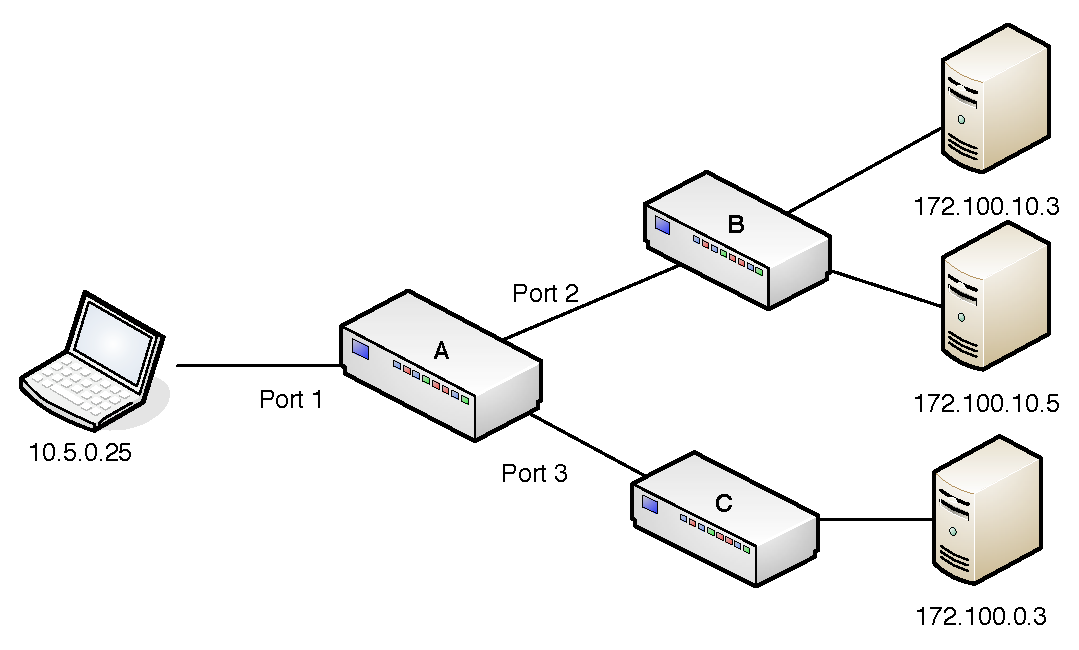
\includegraphics[width=1.0\textwidth]{routing_example_network}
\end{figure}

\begin{enumerate}[1.]
\item The packet leaves 10.5.0.25 and Router A receives it on its interface Port 1.
\item Router A compares the packet's destination \ac{IP} (172.100.10.3) to its table, which looks like Table \ref{tbl:routing_example_routera_table}.
	\begin{table}[h]
	\caption{Routing Example: Router A Table}
	\label{tbl:routing_example_routera_table}
	\centering
	\begin{tabular}{r|c|c|c}
	 & \textbf{\ac{IP}} & \textbf{Mask} & \textbf{Interface}\\
	\hline
	1 & 10.5.0.25 & 255.255.0.0 & Port 1\\
	2 & 172.100.10.0 & 255.255.255.0 & Port 2\\
	3 & 172.100.0.0 & 255.255.0.0 & Port 3\\
	\end{tabular}
	\end{table}
\item Router A determines the \ac{IP} matches best with entry 2, so it sends the packet out on Port 2.
\item Router B receives the packet and does a similar lookup, forwarding it out on the port to 172.100.10.3.
\item 172.100.10.3 receives the packet.
\end{enumerate}

\par This scheme allows a router to direct packets without having to know every individual IP; they only need to know broad address ranges. In the example, Router A possesses no knowledge of how to get the packet directly to 172.100.10.3, but it does know which direction to send it. This becomes exponentially more useful on larger networks. A corporation's network, for instance, may contain hundreds or thousands of addresses, but the routers directing packets to them need only have one entry in their table to correctly route packets. The internal routers of the corporation are then in charge of further routing.

\par This limited-knowledge architecture allows IP hopping to work. As long as table of the routers sending packets in contain the correct \ac{IP} ranges, the systems inside are free to change addresses as frequently as they want and handle internal routing any way they desire.

\subsection{Network Address Translation}
\label{sec:nat}
\par \ac{NAT} is a core technology behind many modern home and corporate networks, allowing many systems to connect to the Internet yet appear to come from a single external \ac{IP} address. A typical home network, for instance, might have the external IP address 184.58.31.151 assigned to it by their \ac{ISP} yet have five systems---laptops, desktops, phones---inside with \acp{IP} like 192.168.0.103, 192.168.0.50, and 192.168.0.1. As these systems send requests out, the router changes the source IP (and port) for packets to the external IP address. As responses come back from the Internet, the router does the opposite, changing the destination of the packets from the external IP to the internal IP of the original requester.

\par To do this, routers must maintain a \ac{NAT} table. This table consists of the source and destination information as well as a new port number, allowing the router to consistently transform traffic in both directions. For example, a router might have a table like the one shown in Table \ref{tab:nat_example}.

\begin{table}
\caption{NAT Table Example}
\label{tab:nat_example}
\centering
\begin{tabular}{r|ccccc}
  & \textbf{Int IP}  & \textbf{Int Port}  & \textbf{Remote IP}  & \textbf{Remote Port}  & \textbf{Ext Port} \\
\hline
1 & 192.168.0.103 & 3547 & 74.125.225.69 & 443 & 50003\\
2 & 192.168.0.103 & 8751 & 207.109.73.34 & 80 & 42630\\
3 & 192.168.0.112 & 30452 & 4.27.2.253 & 80 & 53920
\end{tabular}
\end{table}

\par This small table shows three different connections in progress. The router created each entry the first time the internal system sent out a packet to the remote (Internet) one, for each set of internal and remote \acp{IP} and ports. In addition, the router assigns an external port for each connection to allow it to determine to whom incoming packets are destined.

\par In the future, when the router receives an outgoing packet (from the internal host to the external), it begins by consulting its table to find a match based on the first four values in the table. Based on the table entry, the router changes the source \ac{IP} of the packet to the external IP assigned to it by the \ac{ISP} and the source port to the external port given in the table (if it doesn't find one, it creates a new one). When the router receives a packet from the Internet, it checks for a match in the table based on the remote IP, remote port, and external port. If it finds one, it alters the packet's destination information to the internal IP and port.

\par This system serves two purposes. First, as the number of systems on the Internet has increased, \ac{IPv4} addresses have become a limited resource, with their 32-bit length limiting the number of possible addresses to around four billion. \ac{NAT} allows an organization to only own a single address yet serve many systems behind it. Second, \ac{NAT} inherently acts a simple stateful firewall \cite{DynAddrMalProp}. In order for an outside system to send packets to an internal host, the internal host must initiate the connection, allowing the router to create the table entry.

\subsection{Ethernet and \acf{ARP}}
\label{sec:eth_routing}
\par Many local networks use Ethernet for the first and last leg of network travel to actual hosts. In a flat network, where local machines are connected together via a switch or hub, \ac{IP} routing is not typically used. Instead, packets are directed to the correct recipient via physical identifiers known as \ac{MAC} addresses. Packets sent on an Ethernet network are wrapped in an Ethernet frame, which specifies the \ac{MAC} addresses of the sender and receiver.

\par When a packet is first created, however, the host system only knows the destination \ac{IP}. Before the packet can be sent out, the sender must determine the destination \ac{MAC} address. This is done through a \ac{ARP} request, a process illustrated in Figure \ref{fig:arp_example}.

\begin{figure}[ht]
\caption{\ac{ARP} Example}
\label{fig:arp_example}
\centering
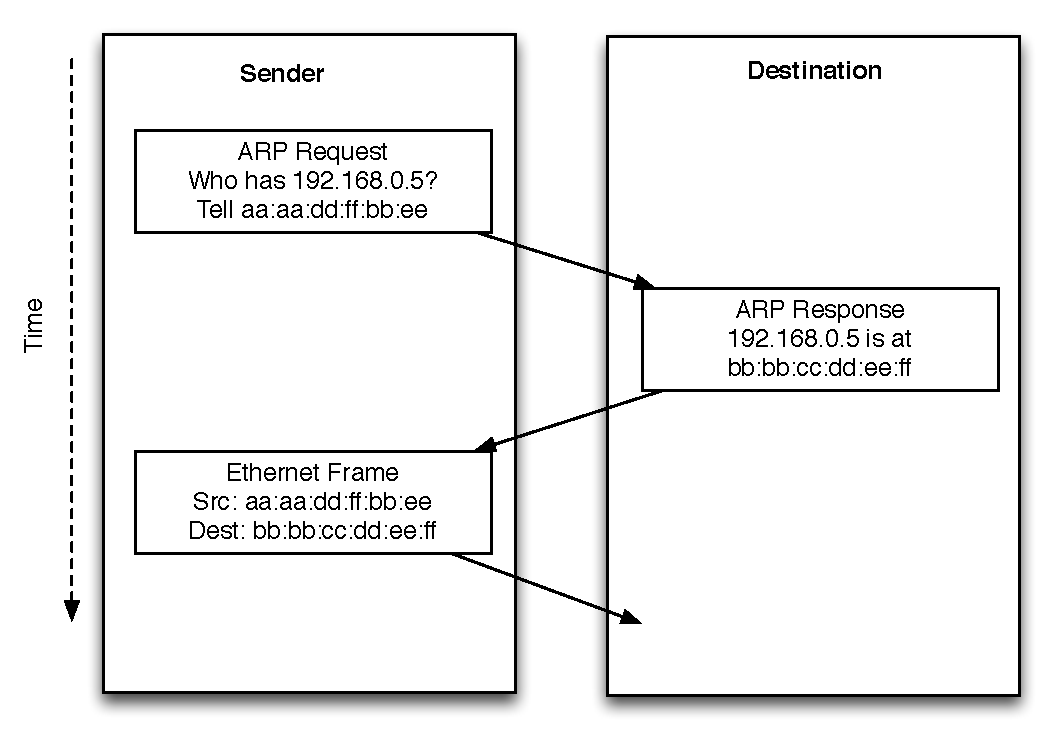
\includegraphics[width=0.8\textwidth]{arp}
\end{figure}

\par As shown, the sender first asks on the network who has the destination \ac{IP}. Every host on the network hears the request, but only the one with that \ac{IP} responds, sending back an \ac{ARP} response with their \ac{MAC} address to the requester. With the destination \ac{MAC} now in hand, the original sender can construct the Ethernet frame for their \ac{IP} packet and send the data on its way. The sender caches the physical address of the other machine for a short time to avoid repeating the \ac{ARP} request too frequently.

\par To send packets beyond the local network, hosts use a gateway system, usually a router. They transfer the packet to the gateway via Ethernet, then the gateway directs the packet further. Ethernet and \ac{ARP} is not used directly by local hosts to reach hosts beyond the gateway.

\section{IP Hopping in Detail}
\label{sec:hopping}
\par Address hopping is a simple concept at a high level: take the basic identifiers of a network and mutate them in a way that only authorized systems understand and continue to use for communication. Doing so makes it difficult for an adversary to correlate sniffed traffic with individual machines and even more difficult to probe into the network to enumerate hosts. Other methods of dynamic network reconfiguration exist, but address hopping may have the greatest potential for obstructing network reconnaissance efforts \cite{DefeatingAdversaryNIE}.

\par In trying to actually implement such a system, however, several issues arise.  The network illustrated in Figure \ref{fig:exnetwork} is used to aid the following discussion. There are two main networks \textit{A} and \textit{B} that are assigned the displayed IP ranges, \tbd{reword: are connected by the Internet, and have an interest in communicating freely with one-another}. Each of these has a few friendly end nodes (\textit{A1}, \textit{A2}, \textit{B1}, etc.) behind a main router (\textit{AR} and \textit{BR}). Additionally, network \textit{B} has a potentially rogue client inside it named \textit{M1}. Outside of those two networks is the friendly \textit{C2} node, who has an interest in at least occasionally communicating with nodes inside networks \textit{A} and \textit{B}, and malicious \textit{M2}, who wants access to said networks. The details of the routes between them and \textit{A} and \textit{B} are inconsequential.

\par Note that for the sake of this discussion non-routable \ac{IPv4} addresses are used. This is done merely for convenience and readability, everything applies to \ac{IPv6} as well, unless otherwise noted.

\begin{figure}
	\centering
	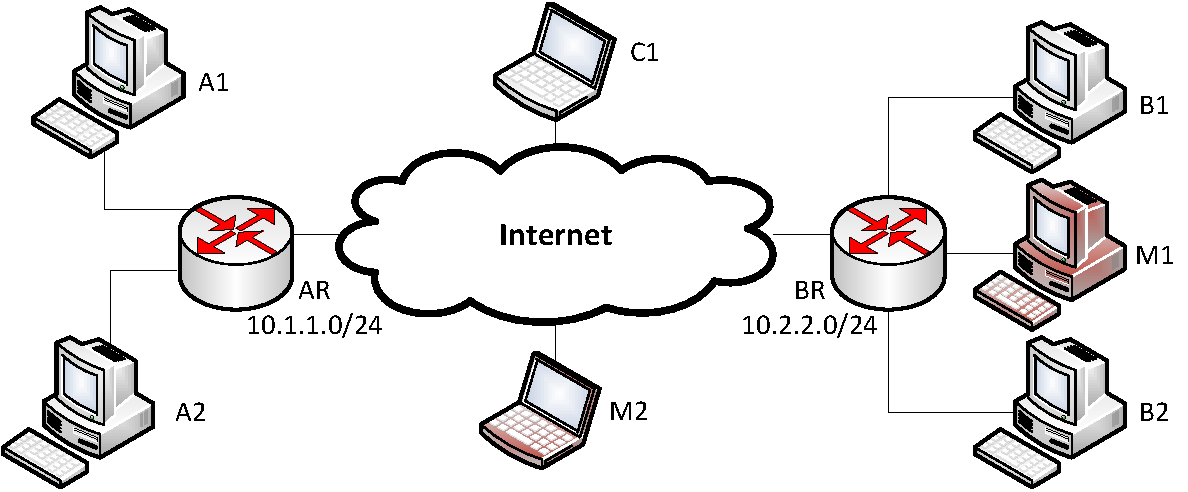
\includegraphics[width=0.75\textwidth]{exnetwork}
	\caption{Example network layout}
	\label{fig:exnetwork}
\end{figure}

\par There are two basic ways to deploy IP address hopping on this network: each end point hops individually or the network gateways transform incoming and outgoing packets. Both options and their strengths and weaknesses are discussed below.

\subsection{End Point Hopping}
\par For the example network, each end point hopping would mean that all of the nodes behind \textit{AR} and \textit{BR} (\textit{A1}, \textit{A2}, \textit{B1}, etc.) change addresses on a periodic basis, independent of one another. Despite the apparent simplicity of this setup, several questions must be answered.

\par First, how do the nodes keep track of one another? If every node knows about all the others, then scalability might become an issue, as every client presumably has to maintain some amount of data on fellow hopping clients to determine where each one is at any given time. It may be possible to devise a scheme where this flaw is mitigated by having all clients hop using the same secret and they each know just the broad IP ranges where fellow hoppers reside (i.e., the \textit{AR} nodes know that 10.2.2.0/24 is a network they talk to with hopping), but this accentuates the next question: how do clients choose their hops?

\par Each node must know some secret from which \ac{IP} addresses are generated, hopefully in a manner which appears random to outsiders yet is predictable for those with the secret. The secret combined with the algorithm used to generate \ac{IP} addresses results in what this thesis refers to as a ``hopping pattern.'' There may be only one of these secrets, which every node in the protected network knows---that is, the nodes in both A and B, hereafter collectively referred to as the ``hopping network.'' This does have the potential flaw of revealing too much information to an eavesdropper though: with a large number of nodes all following a hopping pattern based on the same key, it may be easier to deduce the secret.

\par Giving each node a separate secret would solve this issue. However, each client now has to maintain even more information on every other client. For a small number of nodes this is not a problem, but if the intention is to scale to thousands or tens of thousands of clients problems with processing and key distribution may arise.  

\par Just as importantly, however, is the question of how nodes coordinate their IP address choices. As discussed in Section \ref{sec:routing}, IP routing requires addresses follow a largely hierarchical setup, with broad ranges like 10.0.0.0 leading to 10.1.0.0 to 10.1.1.0 and so on. Thus, if \textit{A} owns the network address range 10.1.1.0/24, then all of its nodes must fall within the address range of 10.1.1.1 through 10.1.1.255. This means that when each node hops it must remain within the valid range of the network to which it connects \textit{and} that the address it chooses must not already be taken another node. Given enough nodes in a subnet, a conflict is quite possible, leading to unpredictable network behavior. 

%\par It is likely possible to devise a reasonably robust algorithm for all nodes to hop simultaneously and end up on unique IPs, but this encounters a few issues with the link-layer of a network's architecture. On local networks, machines are identified by a Media Access Code (MAC) and systems must map IP addresses to the hardware MAC using Address Routing Protocol (ARP). Nodes virtually always cache this information for speed, so for the period of time from a hop to the cache entry expiration time, packets sent to nodes on the local network will likely contain an incorrect MAC and not arrive at the correct destination. TCP would then detect the packet loss and retransmit, trying until either the connection timed out or the ARP cache updated. Even if ARP information is only cached for a few seconds, at best this could result in bursts of traffic on local networks and at worst dropped connections. A similar problem also exists at the switches in the network, although this would likely resolve itself quickly.

%\par It would be possible to work around this issue by having whatever utility is handling the hopping also alter the ARP cache. To do so, every node would need to compute the correct locations of all other nodes and do so at precisely the same time. While not infeasible, this becomes even more platform-specific than the general IP hopping was. Approaching it the other way, nodes could all send gratuitous ARPs when their IP changes, but this still generates extra traffic on the network and \textit{forces} systems to be extremely vulnerable to ARP spoofing, a common part of a network attack.

\par The easiest solution to this problem is to give each node a unique, non-overlapping address range in which to hop. This requires no on-going communication with other nodes to work well and has the distinct advantage of working properly with existing defenses (i.e., a firewall with special rules for a host can point to the range for that host, rather than an individual IP). This setup requires a large enough address space to make hopping beneficial. If a given node only has five possible addresses in which to hop, for instance, it becomes trivial for an attacker to just keep trying a single one until the node returns to it. \ac{IPv6} would alleviate this problem, as the Internet Engineering Task Force recommends the allocation of a /64 address space ($2^{64}$ addresses) to every link \cite{rfc3267}, but \ac{IPv4} with its more limited address space would not allow this flexibility and, unfortunately, the reality of current networks mandates support for \ac{IPv4} \cite{EvaluatingIPv6}. \tbd{see if a paper has an analysis of the needed address space for usability}

\par Of course, with enough coordination between nodes everyone could share the same address space. A fair amount of work would need to be put into an algorithm and protocol to synchronize everyone's changes, but this is not insurmountable. This does break most special cases in firewalls unless the firewall is either made aware of the \ac{IP} hopping system or hosts that need special rules do not change addresses at all.

\par Despite these negatives end point hopping does have advantages. First, scalability issues lie more in storage space and key lookup speed than actual computation, as every node only has to perform packet transformations for their own ingress and egress packets. Although not discussed yet, it is likely that any IP hopping scheme will also incorporate packet encryption, so distributing this load may be beneficial. Second, end point hopping protects clients from probing no matter where the adversary is in the network. For example, as long as \textit{M1} in our example network lacks the hopping key, they have no more of an advantage in scanning any of the \textit{A} or \textit{B} nodes than \textit{M2}, who is outside the network. Finally, end point hopping comes with the ability for individual nodes such as \textit{C1} to easily connect to the main hopping network without the need to develop new software or deploy extra hardware. This is in distinct contrast to gateway-based hopping, which by definition uses a separate system to handle hopping, as Section \ref{sec:gateway_hopping} discusses.

\subsection{Gateway hopping}
\label{sec:gateway_hopping}
\par The alternative to end point hopping is to move the hopping to network gateways. In such a scheme, networks are placed behind gateways that alter all traffic passing through them appropriately. What ``appropriately'' means varies with every implementation, but in one way or another, a gateway outside of the actual end points alters the IP traffic to make it appear as though the systems inside are changing IP addresses. Referring back to the example network in Figure \ref{fig:exnetwork}, gateways \textit{AR} and \textit{BR} would be in charge of these packet transformations, altering traffic from the clients inside their networks (e.g., \textit{A1}, \textit{A2}, etc.) to outside hosts. The secrets at the end point level before are now stored at the gateway, with each gateway getting its own unique set of keys; the gateways typically lack precise knowledge of the end points they protect.

\par Nodes inside the network may or may not have knowledge of the hopping. In most instances the hopping occurs with no modification of the end points and is largely transparent \cite{TAO}. The need to only deploy a small number of gateway systems, rather than altering every client system, gives gateway-based hopping an advantage over end point-based on larger networks. Applying software and/or hardware changes to every system is costly in terms of both time and manpower. Even more significantly, legacy systems running older operating systems might need custom solutions, increasing the cost of deployment.

\par The most common observable side effect of gateway hopping (beyond the latency associated with the additional processing) is \ac{TCP} connection dropping. Because TCP depends on IP addresses and ports numbers to identify on-going connections, any alterations to this information would traditionally kill the connection \cite{NASR}. This is a problem also faced by end point hopping schemes, but is more easily corrected because the individual machines know the state of connections and can correct appropriately. With gateway hopping, however, the situation may require more significant state tracking and packet inspection at the gateway.

\par Because of this required state tracking and the need for a single system to alter all traffic in and out of an entire network, gateway-based hopping presents a possible performance problem. With enough traffic or individual nodes behind a gateway, it may be possible to overload the gateway, leading to dropped packets and failing connections. Depending on gateway design this may be avoided; some studies show a CPU impact of around 10\% (even when encryption is applied) when compared to standard routing \cite{TAO}.

\par Additionally, gateway hopping may have more difficulty accommodating individual clients connecting to the network. In \textit{C1}'s case, for instance, if it wanted to be able to talk to \textit{A1}, it would need to obtain the appropriate hopping information from \textit{AR} and alter its own traffic accordingly. There are several ways to make this work, but all of them require more work than an end-point hopping system would, simply because end-point hopping was already designed around the concept of individual nodes connecting together.

\section{Data Security}
\label{sec:data_security}

\subsection{Hashing}
\label{sec:hashing}
\par Cryptographic hash functions take a given sequence of bytes and return a fixed-length string of bits representing that data. While their output is not unique for every input, cryptographic hashes attempt to make it infeasible to generate two messages with the same hash or to modify an input and get the same hash. As illustrated in Table \ref{tbl:hashing_example}, these properties allow the use of hashes in to verify data because even small changes result in different output.

\begin{table}[h]
\caption{Hashing Example}
\label{tbl:hashing_example}
\centering
\begin{tabular}{r|l|l}
	& \textbf{Input}  & \textbf{Output (SHA-1)} \\
\hline
Original & The quick brown fox jumped & c950af1b07223c7d8590538189b3bcd9f4e08c6c\\
Changed & The quick br\textit{\textbf{a}}wn fox jumped & 97c592d5c0d991b91c68edb3941b1bb075a97f56
\end{tabular}
\end{table}

\par Here even a small change (\textit{o} to \textit{a}) resulted in a significantly different output. If the sender gave both the data and the hash to a recipient, the recipient would be able to repeat the hash on the data and verify that their hash matches the one the sender gave them. Of course, hash algorithms like the \ac{SHA} (used in this example) family are widely published, so anyone can produce a valid hash of any data they want. This means that in and of themselves, hashes do not prevent against malicious modification: an attacker could modify data, then produce a new hash to match. To work around this problem, a digital signature or \ac{HMAC} must be used, as covered in Section \ref{sec:authentication}.

\subsection{Encryption}
\label{sec:encryption}
\par As is discussed in Section \ref{sec:related_research}, encryption is a crucial component of most hopping systems. Additionally, encryption forms the basis of digital signatures and \ac{HMAC}, both means of verifying that a given message---a single packet, in most contexts here---came from where the receiver believes. It is not important for the purposes for this thesis to understand the math behind encryption, but a few concepts are helpful.

\par Encryption comes in two major flavors, symmetric and asymmetric. Symmetric encryption uses the same key for encryption and decryption and, in many cases, is fairly quick. Newer \acp{CPU}, such as Intel's Core processors, include hardware instructions for the commonly used \ac{AES} algorithm, increasing symmetric encryption's speed even further \cite{IntelAES}. Because anyone with the encryption key can decrypt the data, participants must establish their shared secret in a secure way.

\par Asymmetric encryption---also referred to as public-key encryption---provides a way to exchange secure data \textit{without} having to establish a secret key in advance. In asymmetric encryption a public key---known to everyone---and a private key---known only to one participant---are used in conjunction. If a sender wants to transmit data to a specific receiver securely, they encrypt the data with the receiver's public key. When the receiver gets the transmission, they decrypt it with their private key. Because no one else knows the private key of the receiver, it is impossible for anyone else to decrypt the data, even though the encryption key is widely known. In exchange for the robustness and openness of this encryption style, asymmetric encryption algorithms tend to be slow.

\par Asymmetric and symmetric encryption are typically used together in network communications. When a connection is first established, a public-key encryption scheme such as \ac{RSA} determines the shared symmetric key, then all future data is encrypted with a symmetric algorithm like \ac{AES} \cite{HybridEncryption}. This hybrid approach provides the best of both worlds: no need to establish a shared secret in advance and speed during longer communications.

\subsection{Authentication}
\label{sec:authentication}
\par Authenticating that a given sequence of bytes actually comes from whom they say they do can be done through either a \ac{HMAC} \cite{rfc2104} or a digital signature \cite{rfc3447}. These algorithms are based on symmetric and asymmetric encryption, respectively, and therefore share the same strengths and weaknesses. Both algorithms are widely used today in protocols like \ac{IPsec} \cite{rfc2404} and user-level data like email \cite{rfc5751}.

\par \ac{HMAC} works through a series of multiple hashes with the data and an encryption key. Both sender and receiver have the same shared private key, allowing them each to do the \ac{HMAC} process independently. The sender includes their computation of the \ac{HMAC} with the original data, then the receiver calculates their own HMAC and ensures it matches the one sent with the message. If it does, the receiver knows the message is unchanged and comes from someone with the correct shared key.

\par For a digital signature, the sender encrypts the data's hash with their own private key. The recipient verifies the authenticity of the message by performing their own hash of the data and decrypting the signature with the sender's public key. If the calculated hash and the decrypted hash match, the sender must be who they claim to be, as only that sender has access to the correct private key.

\subsection{Combining for Full Effect}
\label{sec:auth_and_encrypt}
\par By combining encryption and authentication, two parties can communication with confidentiality and integrity. For public key encryption, a sender signs the message with their own private key, then encrypts the message with the public key of the recipient \cite{An01authenticatedencryption}. The recipient decrypts the message with their private key, then verifies the signature with the public key of the sender.

\par For symmetric encryption, the opposite order is used. First the sender encrypts the data with one symmetric key, then adds an \ac{HMAC} of the ciphertext \cite{AuthEncrypt}. The receiver computes the \ac{HMAC} of the cipher text and verifies the attached one to ensure the integrity and authenticity of the message. The receiver then decrypts the data.

\section{\acf{TOTP}}
\label{sec:totp}
\par The system discussed in this thesis relies heavily on values that are unpredictable to an outsider but calculable for anyone with the secret key. The algorithm behind these values is \ac{TOTP} \cite{rfc6238}, which in turn relies on the \ac{HOTP} algorithm \cite{rfc4226}. Both of these algorithms are frequently used in the two-factor authentication systems employed by banks and other websites, with a smartphone app or key fob displaying the current password \cite{TwoFactorPhones}.

\par \ac{HOTP} utilizes a key of at least 128-bits and a ``counter'' to produce its output. These are passed to a \ac{SHA}-based \ac{HMAC}, which produces a 20-byte string. It then applies a ``truncation'' process to the \ac{HMAC}, returning a four-byte output \cite{rfc4226}. If both sides of an exchange know the key and the current counter, they are able to independently produce the same value.

\par The counter for \ac{HOTP} is set based on some event that the system designer decides upon. In the most literal case, the usage of a given output for authentication causes an internal counter to be incremented. In a situation like this, both sides of the HOTP (the sender and the receiver) must keep their counters in-sync or the two will produce differing values and need to be resynchronized. In a system with multiple senders and receivers, this becomes quite challenging.

\par To work around this, time may instead be used as the basis of the counter. RFC 6238 defines \ac{TOTP} as a simple extension of \ac{HOTP} where the counter becomes the current time divided by a configured time step \cite{rfc6238}. This change allows all parties interested in a given \ac{TOTP} to produce the same value as long as they keep their clocks relatively similar (within one time step). 

\section{Previous Implementations}
\label{sec:related_research}
\subsubsection{BBN's \acf{DYNAT}}
\par BBN Technologies' 2001 paper entitled ``Dynamic Approaches to Thwart Adversary Intelligence Gathering'' tests the hypothesis that ``dynamic modification of defense structure improves system assurance'' \cite{BBNDYNAT}. In the paper they lay out a custom address space randomization solution called \ac{DYNAT}.

\par A series of red-team experiments tests against their \ac{DYNAT} were used to test if the addition of \ac{IP} hopping decreases an adversary's ability to map the network. The experimentation confirm BBN's hypothesis: DYNAT does increase system assurance because the adversary's work greatly increases in comparison to static networks. Even when the red team receives intimate knowledge of the DYNAT's operation, the adversary could not identify a critical server in an enclave with DYNAT active.

\par The BBN's implementation focuses on individual clients connecting to a server enclave through a DYNAT gateway on the server end. This gateway transforms incoming and outgoing packets between ``true'' host identification information---e.g., the actual \ac{IP} address and port number of a server inside the enclave's network---and values which vary based on a pre-shared key and time. On the client side, a ``DYNAT shim'' sits in the network stack and did the same thing, transparently allowing client applications to work with the server enclave. Additionally, DYNAT applies encryption to all traffic for confidentiality.

\par BBN's experiments also found that encryption of the packets is crucial, as the attackers can trivially sniff the traffic to find important servers, even if they do not know the real IP address or port of the target. For example, an attacker might see a packet containing an \ac{HTTP} response and thus learn an active IP and port for a web server, even if probing for it is impossible. While this information remains valid for a limited period, it may give enough time for the attacker to compromise the internal network.

\subsubsection{Sandia Dynat}
\par Sandia National Labs' 2001 final report on their extensive work in the ``dynat'' field examines virtually every detail in \ac{IP} hopping systems, from how hopping is synchronized to where in the network it is implemented \cite{SandiaDynat}. This paper points to many of the important issues that must be considered when implementing or deploying an \ac{IP} hopping tool.

\par Of note are Sandia's recommendations on the location of the deployment of a gateway-based \ac{DYNAT}. In order to avoid interference with existing firewall rules---particularly ones with a stateful firewall---, a hopping gateway must be deployed beyond the current system. Likewise, for gateway-based \acp{VPN}, there is often a static \ac{IP} requirement to allow for authentication \cite{SandiaDynat}, so a IP hopping gateway must also lie beyond the \ac{VPN} concentrator, closer to the public-facing side of the network. Essentially, the hopping gateway should be the last system before each the network connects to the outside world \cite{SandiaDynat}.

\par The Sandia report also provides significant insight into the interaction of a \ac{DYNAT} with \ac{IPsec} and strongly suggests a combination of the two. First, the encryption from \ac{IPsec} avoids the ineffectiveness of address space randomization if the packets can be trivially sniffed for information, as BBN's work reveals \cite{BBNDYNAT}. Second, a \ac{DYNAT} strengthens \ac{IPsec}, as the hopping gateway can quickly reject invalid packets based on invalid source and destination identifiers, rather than forcing IPsec to perform expensive \ac{HMAC} computations and/or encryption. However, the report also warns that the use of IPsec with a hopping gateway can reduce some aspects of \ac{DYNAT}'s access control because more identifiers are encrypted and unusable.

\subsubsection{\acf{APOD}}
\par BBN continued work in the dynamic network address translation field and proposed another IP hopping implementation in 2003 as part of the \ac{DARPA} \acf{APOD} project \cite{APOD}. This system is a refinement of their previous \ac{DYNAT}, featuring a \ac{NAT} gateway sitting either on the server host itself or on a gateway into the network.

\par The primary differences between APOD and the previous DYNAT relates to implementation. Whereas the BBN DYNAT is a very specialized solution, \ac{APOD} employs standard \ac{COTS} utilities, such as Linux's iptables, to perform much of its work. This paper proposes the use of a \ac{NAT} gateway on the networks of both the client and the server, rather than a gateway only at the server side and/or specialized software on each end point.

\subsubsection{\acf{NASR}}
\par The 2005 \acf{NASR} is an \ac{IP} address hopping system designed to defeat hitlist-based worms \cite{NASR}. These worms spread to pre-collected lists of \ac{IP} addresses and typically propagate much faster than traditional worms that target random \acp{IP}. To fight this, \ac{NASR} causes the pre-built hitlists to decay by changing IP addresses on a periodic basis.

\par The most unique aspect of this research is the use of \ac{DHCP} to force the changes. Through the use of a slightly intelligent \ac{DHCP} server that leases \acp{IP} for a only a short time frame (on the order of tens of minutes) and only offers \acp{IP} that have not been used recently, most networks already using DHCP can quickly change to a randomized scheme. This simplicity does come at a cost, however: \ac{TCP} connections die whenever the IP change occurs, forcing the hopping period to be quite long or risk unacceptable connection losses.

\par \ac{NASR} attempts to reduce this issue by introducing additional intelligence into the DHCP server to allow it to detect ``long-lived'' TCP connections (i.e., a download) and give clients the same IP if they appear busy. Beyond that, they also monitor what services each client uses, as many are resilient to a connection being torn down \cite{NASR}. Despite those improvements, address changes occur even in the fastest of instances only once an hour or so. As tests show, this meets the goal of hitlist worm protection, but is likely inadequate for obfuscating the network from a more intelligent, focused enemy.

\subsubsection{\acf{NAH}}
\par A 2005 paper by European researchers presents a system they call \acf{NAH} \cite{NAH}. This system focuses on a client contacting a server as a negotiable protection measure, rather than an always-on system used between pre-configured systems.

\par A protocol employing \ac{IPv6} allows a client to tell a server that they supported (and wish to use) \ac{NAH}. If the server supports NAH, it replies with its hopping pattern. The client then sent its own hopping pattern, before reconnecting using the pattern the server just gave it. Hops occur based on packet count per connection, rather than a time-based factor.

\par Once again, the NAH authors note the importance of encryption in maintaining the confidentiality of the data stream. However, they also state that without encryption the system still provides some benefit, as packets bound for ``different'' addresses might follow differing network routes due to the different (perceived) destinations. If this occurs, an attacker needs to either compromise a route fairly close to an endpoint to ensure they see all traffic or compromise every possible route and collate the traffic together. Even if they manage to accomplish that, the attacker would still have to collect all traffic passing them in order to reconstruct the full stream (because they are unable to filter for specific \acp{IP} to identify the connection they are interested in), which poses a storage and computation problem given enough data \cite{NAH}.

\par As an additional side effect of the variable routing, the researchers noted that such a system may actually increase the throughput and reliability of a system. If multiple routing paths are used, the network may avoid congestion and allow traffic to flow more smoothly \cite{MultimediaDistributed}. While this is not an important aspect of this system, the potential does add support to the employment of address hopping \cite{NAH}.

\subsubsection{\acf{TAO}}
\par The 2006 \ac{TAO} focuses on protection of the Internet as a whole from hitlist-based worms and is somewhat based on the previous work in \ac{NASR} \cite{NASR}. It features gateways on networks that maintain external-to-internal address mappings for all nodes inside the protected network, with the external addresses changing with a configurable frequency. To maintain existing connection regardless of mapping changes, TAO include a \ac{NAT} table. 

\par A disadvantage of this design came in the form of address space overhead, because each individual box receives a publicly accessible \ac{IP} and the \ac{NAT} table claims additional \acp{IP} for on-going connections. Testing shows that around 10\% more address space is needed for three simulations on large-scale networks. However, \ac{TAO} has the distinct advantage of only requiring the addition of a single box at the network's edge and no cooperation from remote hosts is needed for it to provide its services.

\section{Summary}
\label{sec:background_summary}
\par This chapter presents background topics used in this thesis, including \ac{IP} routing, encryption and authentication, and \aclp{TOTP}. \ac{IP} hopping and the two possible approaches to it---end point or gateway---are discussed, along with an analysis of each of their benefits and challenges. Finally, previous research in this area is covered.


\chapter{Implementation}
\label{chp:implementation}

\par The research this thesis presents relies on a custom \ac{IP} address hopping solution. This chapter covers many of the details of this system, from high-level architecture to the network protocol. Section \ref{sec:arg_requirements} covers the requirements this system strives to meet. Section \ref{sec:arg_impl_overview} gives an architecture overview, while Section \ref{sec:arg_components} covers the details of each component in the system. Section \ref{sec:arg_protocol} details the network protocol used by the system to coordinate gateways.

\section{Requirements}
\label{sec:arg_requirements}
\par \ac{ARG} focuses on the needs of military networks. These are essentially the needs of any geographically-diverse organization: locations throughout the world, high availability and reliability requirements, and security over any network through which its data travels \cite{DialInNetworking}.

\par ARG primarily attempts to protect communication outside of military-controlled networks and prevent external entities from probing internally. This protection includes privacy, as \ac{ARG} (like any network address space randomization tool) helps hide information from adversaries by obfuscating sender and receiver information \cite{NetworkBasedPrivacy}. This means that the implementation described is intended to be employed for all traffic traveling between bases, but is unconcerned with internal base traffic. Internal network defense remains the purview of traditional defenses. Base networks, in this case, include both those on permanent installations and those in deployed, forward locations. 

\par ARG must operate over the commercial Internet. Some proposals for network address space randomization require changes to the Internet's existing routing infrastructure and protocols \cite{CONTRA, APOD}. Deploying such a solution may be possible and beneficial in the long run, but a solution that could be deployed today without participation from outside entities is more feasible. This is especially true for forward locations, where traffic is more likely to utilize infrastructure outside the military's control.

\par Like any large, distributed organization, bases can generate huge volumes of traffic, so ARG must scale well. Due to the importance of networks to command and control, ARG's implementation must not introduce significant latency under any foreseeable load. Likewise, there can never be a brief period where all connections drop. At a minimum, given the number of nodes inside the network, dropped connections result in a massive amount of wasted bandwidth as they are reestablished and the data retransmitted.

\par Military networks contain a wide range of hardware and software. Much of this software cannot be altered to accommodate \ac{ARG}, so it must function transparently. Host-level implementations might be feasible for generic workstation images (i.e., an alteration to the operating system's network stack), but the ability to function in another way must exist to allow legacy equipment to continue operating.

%\par Finally, resource constraints---monetary and manpower---preclude some options. ARG is intended to be easily configurable and usable with reasonable hardware investments. ARG requires only a single gateway system for each network it is intended to protect, rather than hardware and/or software for every client inside those networks.

\section{Architecture Overview}
\label{sec:arg_impl_overview}
%\par Based on these requirements and the previously cited literature, this paper proposes the Address Routing Gateway. While actual testing of this setup is beyond the scope of this paper, we will attempt to analyze the advantages it would provide, based on previous experimentation.

\par As illustrated in Figure \ref{fig:arg_concept_network}, \ac{ARG} functions entirely around standard networks with hopping gateways. This matches the ``gateway hopping'' scheme discussed in Section \ref{sec:gateway_hopping}. As with \cite{TAO}, these gateways are standalone systems, not intended for use with other tasks. Individual hosts inside these networks have no knowledge of the traffic transformations the gateways perform, whether their connections are routing to a host inside the local network, to a host inside another associated hopping network (hereafter referred to as an ``ARG network''), or to an external network. The implementation of ARG allows the deployment of standard passive defense technologies like firewalls inside the network without reconfiguration. Each gateway maintains a \ac{NAT}-like table to ensure that existing connections are maintained across hops (essentially temporarily leaving the old IP active for just those connections using it already).

\begin{figure}
	\centering
	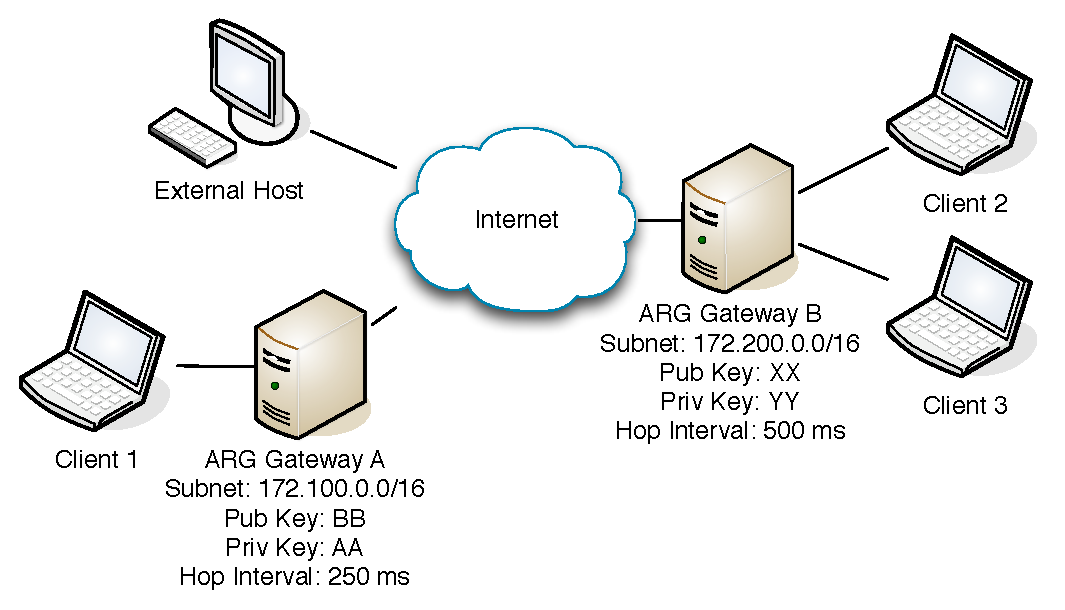
\includegraphics[width=1\textwidth]{arg_concept_network}
	\caption{\ac{ARG} conceptual network layout}
	\label{fig:arg_concept_network}
\end{figure}

\par Each gateway is given what subnet it is permitted to hop within, a private/public key pair, and time it should wait between \ac{IP} address changes (frequently referred to as its ``hop interval''). For example, \ac{ARG} Gateway A in Figure \ref{fig:arg_concept_network} uses subnet 172.100.0.0/16, has the specified public and private keys, and hops every 250 milliseconds. Additionally, each gateway is pre-configured with knowledge of at least one other gateway. The configured information consists solely of the subnet the other gateway is handling and a public key to use for authentication with it. In the figure, this would mean that Gateway A knows that Gateway B sits in the 172.200.0.0/16 subnet and has the public key XX, but nothing else. The gateways transfer additional information during the connection process. 

\par At startup, each gateway generates a random symmetric encryption key and a ``hop key.'' They then attempt to connect to all other gateways for which they have configuration files through a series of data and time synchronization packets. Once two gateways fully connect, they exchange data about all other gateways they have configured, allowing \ac{ARG} nodes to connect to gateways for which they do not have physical configuration files. Periodically gateways re-send time synchronization information, ensuring that changing network conditions do not kill communication. Section \ref{sec:arg_protocol} and Appendix \ref{chp:protocol} cover each of these packet exchanges in more detail.

\par Once connected, packets between ARG networks are encapsulated, encrypted, and authenticated by the originating network's gateway, with each packet given the destination network's current \ac{IP} address. On receipt, a gateway checks that the \acp{IP} match what they expect (both its own IP and the source's IP), then validates the authentication information (signature/\ac{HMAC}) before forwarding the original packet into their network. Packets to external hosts flow through the \ac{NAT}-style system covered in Section \ref{sec:arg_nat}. 

\par During the evaluation of \acp{IP}, gateways allow packets to match either the current address or the previous one. This allows packets sent just before an \ac{IP} change to still be accepted. If a gateway's hop interval is shorter than twice the one-way latency, packets will never be accepted, as illustrated in Figure \ref{fig:late_packet_example}. In this figure, Gate A sends a packet to Gate B with the destination addresses set to the current \ac{IP} at that time (172.200.210.85). The packet takes 50 milliseconds to travel across the network, during which time the gateways change addresses twice. When the packet reaches Gate B it is rejected, because the packet's destination \ac{IP} does not match the current (172.200.38.138) or previous (172.200.60.97) \acp{IP}.

\begin{figure}
\caption{Packet sent between gateways when hop interval is half the latency}
\label{fig:late_packet_example}
\centering
\noindent\makebox[\textwidth]{%
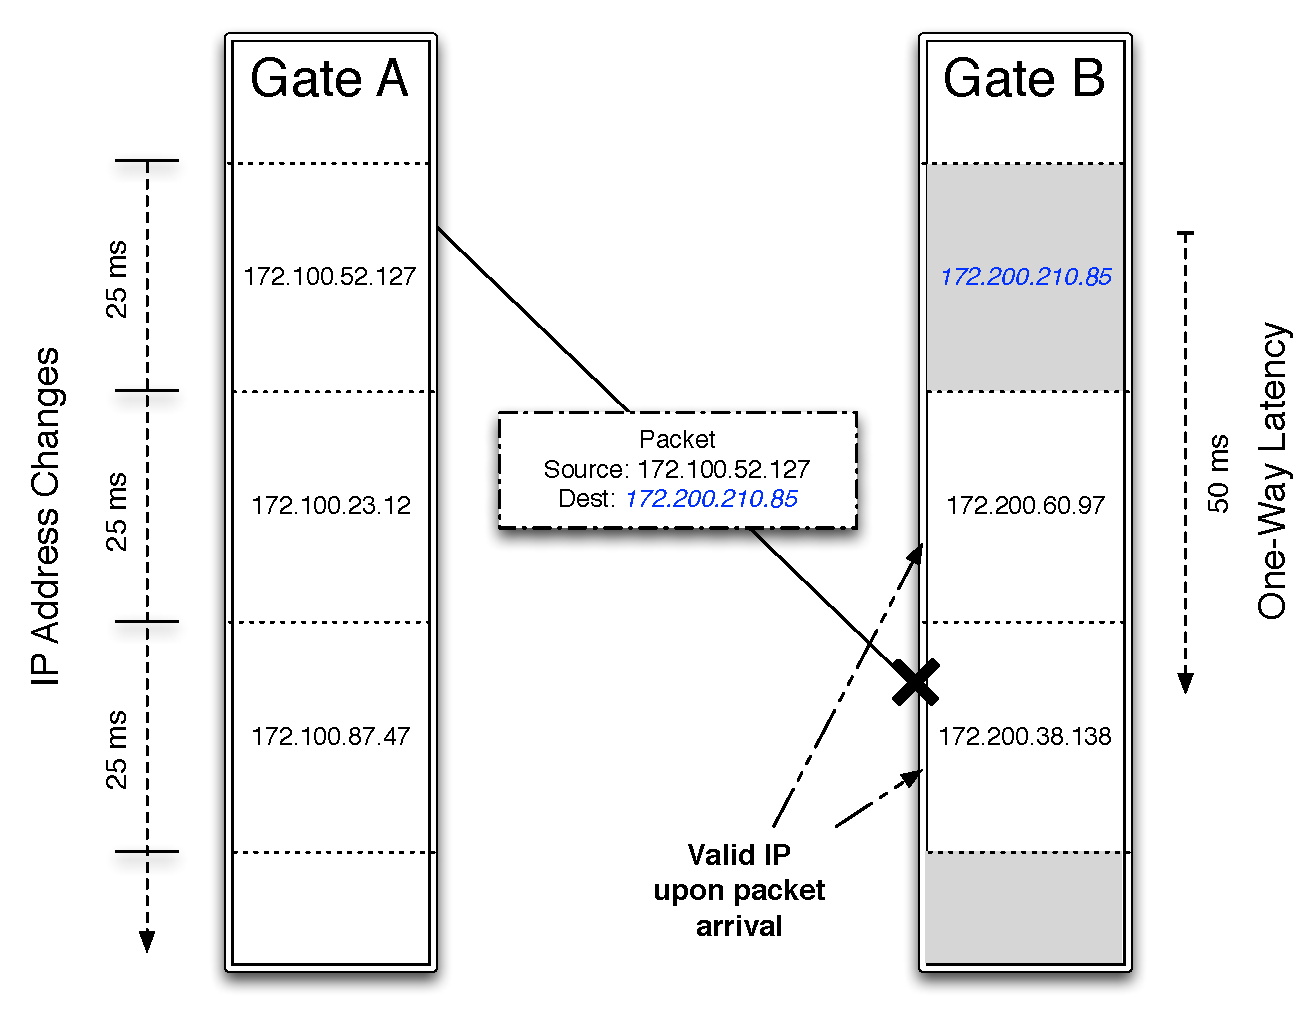
\includegraphics[width=1.2\textwidth]{late_packet_example}
}
\end{figure}

\section{Components}
\label{sec:arg_components}
The handling of packets within ARG is distinctly different if they are to an external (non-ARG network) host or to an ARG network. These processes are handled by two separate components, the hopper and the NAT. A high-level director decides which of these two receives each incoming packets. All of these components run as separate threads on the same gateway, closely coordinating their work. Because it is in charge of overall system operation, this section begins by discussing the director.

\subsection{Director}
\label{sec:arg_director}
\par The director is in charge of receiving packets on the internal and external interfaces of the gateway. Upon receipt of a packet, the director parses the packet and decides how to handle it. The director's decision tree is illustrated in Figure \ref{fig:arg_director_flow} and discussed below.

\begin{figure}
\caption{\ac{ARG} director flow}
\label{fig:arg_director_flow}
\centering
\includegraphics[width=1.0\textwidth,clip=true,trim=0 0 0 0]{flow_director}
\end{figure}

\par In the case of \ac{ARP} requests on either interface, the director replies with the gateway's \ac{MAC} address. This feature of \ac{ARG} allows its use without any changes to the network it is placed in, as hosts continue to send to the ``same'' gateway IP as before and \ac{ARG} responds, despite not technically possessing an internal \ac{IP} of its own. For example, the inside hosts send out an \ac{ARP} request for their normal \ac{IP} gateway (as Section \ref{sec:eth_routing} discusses) and the \ac{ARG} gateway sends an \ac{ARP} response, allowing it to grab all traffic and process it appropriately. More details on Ethernet and \ac{IP} routing can be found in Sections \ref{sec:eth_routing} and \ref{sec:ip_routing}.

\par For outgoing packets (packets that are sent from within the protected network that are intended to leave the network), the director checks the destination \ac{IP} of the packet. If the IP is unknown, it is passed to the \ac{NAT} module. If the IP is within another \ac{ARG} network the director knows, the packet is handed off to the hopper module to be wrapped and transmitted.

\par For incoming packets (packets hitting the external interface), the director first checks if the source IP is another ARG network. If it is \textit{not}, the director quickly hands the packet off to the NAT inbound handler.

\par If the packet \textit{is} from another ARG network, the director checks if the packet type indicates it is an administrative packet and hands it off to the hopper's administrative processor. If it is not an administrative packet, the director confirms the gateway which sent the packet is actually connected. Which gateway is determined by matching the source \ac{IP} to the base \ac{IP} and mask in the local gateway's configuration. Assuming that the gateway is connected, the local gateway checks that the source and destination \acp{IP} are correct, based on the data the hopper has on the other gateway. Assuming all checks pass, the packet is handed off to the hopper to be unwrapped and forwarded into the network. If any fail, the packet is silently dropped.

\subsection{Hopper}
\label{sec:arg_hopper}
\par The hopping module is the heart of ARG. It maintains the state of the gateways (e.g., keys, hop intervals, times) it knows about and transfers packets to and from the network it is protecting. The other two components (director and \ac{NAT}) talk to the hopper to obtain current IP information and if a given gateway is connected or not. 

\par When the hopper first starts, it initializes a list of gateways with data from configuration files. The information maintained in this structure is shown in Table \ref{tab:gatestate}. 

\begin{table}
\caption{Information hopper module maintains on other \ac{ARG} gateways}
\label{tab:gatestate}
\centering
\begin{tabular}{ll}
\toprule
	\textbf{Data} & \textbf{Information Source}\\
	\hline
	IP Range (IP and mask) & Configuration file (see Appendix \ref{chp:argconf})\\
	\ac{RSA} Public Key & Configuration file\\
	Hop Interval & Transferred during connection (see Section \ref{sec:arg_protocol})\\
	Symmetric Key & Transferred during connection\\
	Hop Key & Transferred during connection\\
	Time Base & Calculated based on latency (see Appendix \ref{chp:protocol})\\
\bottomrule
\end{tabular}
\end{table}

\par An administrative thread is started at the same time. This thread attempts to connect to each gateway in its list periodically and, if it does not hear from a given gateway for several minutes, marks gateways as disconnected. In addition, it sends periodic time synchronization requests to connected gateways, especially if it sees a large percentage of packets being rejected due to incorrect \ac{IP} addresses. 

\par Beyond the administrative thread, actions occur in the hopper only when the director passes packets off to it. Outgoing packets are always wrapped, encrypted, and signed, as covered under the ``route packet'' process in Section \ref{sec:arg_protocol_route}. Incoming packets go through the validation process shown in Figure \ref{fig:arg_hopper_in_validation} before being handled. Note that \ac{IP} checking is done in the director before control reaches the hopper. After validation exact handling depends on the packet type, but is generally covered in Section \ref{sec:arg_protocol} as part of the protocol discussion.

\begin{figure}
\caption{\ac{ARG} incoming packet validation process}
\label{fig:arg_hopper_in_validation}
\centering
\includegraphics[width=1.0\textwidth,clip=true,trim=0 0 0 0]{flow_packet_validation}
\end{figure}

\subsection{Network Address Translator}
\label{sec:arg_nat}
\par The \ac{NAT} component of \ac{ARG} maintains a list of on-going connections to external hosts. For instance, if a client inside a protected network connects to 72.246.189.120, the \ac{NAT} creates an entry in an internal table and allows packets from the external host back in to the network and to the client. This is almost identical to the operation of the basic \ac{NAT} discussed in Section \ref{sec:nat}. The only difference from a normal \ac{NAT} system is the addition of an extra field in the \ac{NAT} table for the \ac{IP} at the time the connection was first established. The new version of the table with example data is shown in Table \ref{tab:arg_nat_example} with the new column in italics.

\begin{table}
\caption{\ac{ARG} \ac{NAT} table example}
\label{tab:arg_nat_example}
\centering
\noindent\makebox[\textwidth]{%
\begin{tabular}{rcccccc}
\toprule
  & \textbf{Int IP}  & \textbf{Int Port}  & \textbf{Remote IP}  & \textbf{Remote Port}  & \textbf{\textit{Ext IP}}  & \textbf{Ext Port} \\
\hline
1 & \texttt{192.168.0.103} & 3547 & \texttt{74.125.225.69} & 443 & \textit{\texttt{172.1.123.35}} & 50003\\
2 & \texttt{192.168.0.103} & 8751 & \texttt{207.109.73.34} & 80 & \textit{\texttt{172.1.73.1}} & 42630\\
3 & \texttt{192.168.0.112} & 30452 & \texttt{4.27.2.253} & 80 & \textit{\texttt{172.1.86.173}} & 53920\\
\bottomrule
\end{tabular}}
\end{table}

\par The traditional \ac{NAT} processing and logic is supplemented with this additional information. When a packet goes out, the table is checked and the packet has its source \ac{IP} address and port changed to the external values. If this is the first packet in a connection, the external IP is filled from the current \ac{IP} of the gateway. When an incoming packet is encountered, the external IP and port are both checked to determine the correct internal host. The addition of the external IP to the table allows connections to survive across hops; many connections last longer than \ac{ARG}'s intended hop rate and severing connections frequently is unacceptable for many applications. 

\section{\ac{ARG} Protocol}
\label{sec:arg_protocol}
\par The \ac{ARG} protocol is designed to be fairly stateless, simplifying the implementation and lowering the likelihood of an exploit forcing the gateway into an unexpected state. \ac{ARG} sends data between gateways as the direct payload of the \ac{IP} packet; transport-layer protocols such as \ac{UDP} and \ac{TCP} are not used. If needed, the protocol could be adapted easily to work as a \ac{UDP} payload. \ac{ARG} packets are identified by \ac{IP} protocol 253, a protocol reserved for experimentation \cite{rfc3692}. All packets sent between \ac{ARG} gateways use the header structure shown in Table \ref{tab:arg_packet_structure}.

\begin{table}
\caption{\ac{ARG} packet data}
\label{tab:arg_packet_structure}
\centering
\begin{tabular}{lll}
\toprule
\textbf{Data} & \textbf{Size} & \textbf{Data Type}\\
\hline
Version & 1 byte & Unsigned Integer\\
Message Type & 1 byte & Enumeration, see Table \ref{tbl:arg_protocol_types}\\
Message Length & 2 bytes & Unsigned Integer\\
Sequence Number & 4 bytes & Unsigned Integer\\
Signature & 128 bytes & Raw\\
Payload & 0-32,629 bytes & Message-type specific, see Appendix \ref{chp:protocol}\\
\bottomrule
\end{tabular}
\end{table}

\par For this research, the protocol version field is set to 1 at all times. The type field tells the receiving gateway how to process the data contained in the message. Possible values are shown in Table \ref{tbl:arg_protocol_types}. More details on the format of each message type are given in Appendix \ref{chp:protocol}. Length is the network-order size in bytes of the data from the version to the end of the data; given the size of the message header, the minimum for this is 136. The sequence number is a monotonically increasing unsigned integer value used to prevent replay attacks.

\begin{table}
\caption{\ac{ARG} message types}
\label{tbl:arg_protocol_types}
\begin{tabular}{lcl}
\toprule
\textbf{Mnemonic} & \textbf{Value} & \textbf{Description}\\
\hline
\texttt{WRAPPED} & 1 & Encapsulated packet from protected client to protected client\\
\texttt{PING} & 2 & Time synchronization message\\
\texttt{CONN\_RESP} & 3 & Connection data response message\\
\texttt{CONN\_REQ} & 4 & Connection data and request for other gateway's data\\ 
\texttt{TRUST\_DATA} & 5 & Configuration information \\
\bottomrule
\end{tabular}
\end{table}

\par The signature field may actually contain two possible values: a true \ac{RSA} digital signature of the packet or an \ac{HMAC} of the packet, depending on the message type. Packets of type \texttt{PING} or \texttt{CONN\_REQ}/\texttt{CONN\_RESP} are encrypted with the public key of the receiver and signed with the private key of the sender. All other packets---types \texttt{WRAPPED} and \texttt{TRUST\_DATA}---are encrypted with the symmetric key of the receiver and include an \ac{HMAC} of the encrypted data using with the symmetric key of the sender, following standard encrypt-then-MAC practice \cite{AuthEncryptThenMAC}. The encryption and signing combinations used for each message type as well as whether or not the source and destination \ac{IP} addresses are strictly checked are summarized in Table \ref{tbl:arg_protocol_security}.

\par As a side note, the encrypt-then-sign order used by \ac{ARG} (when using a digital signature rather than an \ac{HMAC}) is backwards according to best-practice \ac{RSA} and should be corrected to sign-then-encrypt \cite{RobustPrinciplesPK}. It may also be wise to add the name of the sending gateway to each message to help prevent similar mistakes in the future \cite{EngPricCrypto}. The order \ac{ARG} uses allows an attacker to sign a message and claim it as their own \cite{rfc2633}. However, \ac{ARG} gateways will still reject these falsified messages because the receiving gateway will not have a public key for the signer. A gateway could successfully sign another gateway's message, but this indicates a compromised of the gateway itself, at which point the attacker has full access to the entire network anyway.

\begin{table}
\caption{\ac{ARG} message security summary}
\label{tbl:arg_protocol_security}
\centering
\begin{tabular}{llll}
\toprule
\textbf{Type} & \textbf{Encryption} & \textbf{Signing} & \textbf{\acp{IP} checked?}\\
\hline
\texttt{WRAPPED} & AES, remote key & HMAC, local key & Yes\\
\texttt{PING} & RSA, remote public key & Signature, local private key & No\\
\texttt{CONN\_RESP} & RSA, remote public key & Signature, local private key & No\\
\texttt{CONN\_REQ} & RSA, remote public key & Signature, local private key & No\\
\texttt{TRUST\_DATA} & AES, remote key & HMAC, local key & No\\
\bottomrule
\end{tabular}
\end{table}

\par There are four basic exchanges that happen between \ac{ARG} gateways: connect, time synchronization, trust data exchange, and packet transfer. In order for gateways to begin exchanging packets between the networks they are protecting (via the ``route packet'' process), they must first fully connect by completing the connect and time synchronization processes. The trust data exchange step is optional, although it allows gateways to connect to others without configuration files. The precise requests, receives, and verifications for each exchange are given in Appendix \ref{chp:protocol}.

\section{Summary}
\par This chapter discusses the implementation of \ac{ARG}. It begins with the requirements \ac{ARG} fulfills, then covers the high-level architecture of the system. The chapter then examines each component and the protocol \ac{ARG} uses between gateways.


\chapter{Methodology}
\label{chp:methodology}

\par This chapter discusses the methodology used to measure the effectiveness of \ac{ARG} at correctly classifying valid and invalid traffic, the maximum supportable hop rate at various network latencies, the maximum packet rate \ac{ARG} can handle, and the overall stability of the system under test. Section \ref{sec:problem_def} discusses the problem this research seeks to answer. Section \ref{sec:boundaries} defines the \ac{SUT} and Section \ref{sec:services} goes into detail on the possible outcomes of the \ac{CUT}. Section \ref{sec:workload} covers the workload presented to the \ac{SUT}, Section \ref{sec:metrics} covers the metrics collected, and Section \ref{sec:parameters} covers the configurable parameters of the \ac{SUT}. Section \ref{sec:factors} brings the previous sections together, giving a comprehensive list of the factors varied for each test. Section \ref{sec:exp_design} details the actual tests and the purpose of each.

\section{Problem Definition}
\label{sec:problem_def}
\subsection{Goals and Hypothesis}
\label{sec:goals}
\par This research seeks to test whether network address space randomization is suitable for deployment on a military network, as Chapter \ref{chp:implementation} discusses. Tests against this system are designed to answer four basic questions:

\begin{enumerate}
\item Does \ac{ARG} classify traffic correctly? What percentage of false positives (valid packets blocked) and false negatives (invalid traffic allowed through) does it introduce?
\item What is the max packet rate and throughput \ac{ARG} can handle?
\item What is the max hop rate---the frequency with which \ac{ARG} changes \ac{IP} addresses---that still allows for reliable communication? How does latency affect this?
\item Is \ac{ARG} stable when presented with corrupt, malformed, or replayed packets?
\end{enumerate}

%\par The software developed and tested here attempts to interfere minimally with the network, a critical requirement for the real-world deployment of such technology. Systems \ac{ARG} touches---both inside and outside the ``protected'' networks---do not need any modifications to continue to function. The research done here provides data on whether this is true as a side effect, potentially valuable information for an organization considering employing a \ac{DYNAT} solution. However, validation of this design goal is not a primary objective. 

%\par The working hypothesis for this research is, as speculated by Sandia, a \ac{DYNAT} system allows for quick identification of unexpected (and potentially malicious) packets entering a network. There are few identifiers within the scope of \ac{DYNAT} by which outgoing packets could be filtered. Given that, no filtering is done for outbound packets and hence no change in behavior is observed when compared to the control network. 

\par It is hypothesized that \ac{ARG} correctly classifies 99\% of traffic it encounters when operating with a hop rate appropriate for the network latency. In addition, this thesis hypothesizes that packet loss become acceptable when the hop rate matches or exceeds the network latency, where acceptable loss is defined as less than 2\%. (This percentage is based on the loss seen on Massachusetts Institute of Technology's wireless networks \cite{MITWifiLoss}.) The other two questions under test are informational in nature as the results apply only to this specific hopping gateway implementation, but it is believed that \ac{ARG} is stable in the face of malformed traffic and it can handle at least 10 \ac{Mbps} of traffic. 

\subsection{Approach}
\label{sec:approach}
\par This research is done on a test network with nodes representing the types of hosts found on a typical, corporate-style network. These include trusted hosts inside trusted networks which communicate freely, internal and external servers that must be accessible to hosts inside these trusted networks, and malicious hosts outside the networks. A configurable custom hopping gateway sits in front of the trusted networks. 

\par Traffic generators and collectors run on the test network, determining which traffic flows successfully make it to their intended destination. This includes examining both false positive and false negative rates, determining why \ac{ARG} rejects packets that should get through and why it allows packets that should be rejected. After a given test, logs and traffic captures are collated to form a complete picture of the traffic on the network before determining statistics.

\FloatBarrier
\section{System Boundaries}
\label{sec:boundaries}
\par The \ac{SUT} is \ac{ARG}, the custom \ac{IP} hopping gateway developed specifically for this effort. The basic components of this system, the various inputs into the system, possible outputs, and the metrics provided are illustrated in Figure \ref{fig:sut}. The sections following cover aspects of this diagram in more detail, with Section \ref{sec:services} discussing the possible outcomes, Section \ref{sec:workload} covering the workload, Section \ref{sec:parameters} detailing the parameters in use, and Section \ref{sec:metrics} covering the metrics collected.

\begin{figure}
\caption{\ac{ARG} \ac{SUT} diagram}
\label{fig:sut}
\centering
\noindent\makebox[\textwidth]{%
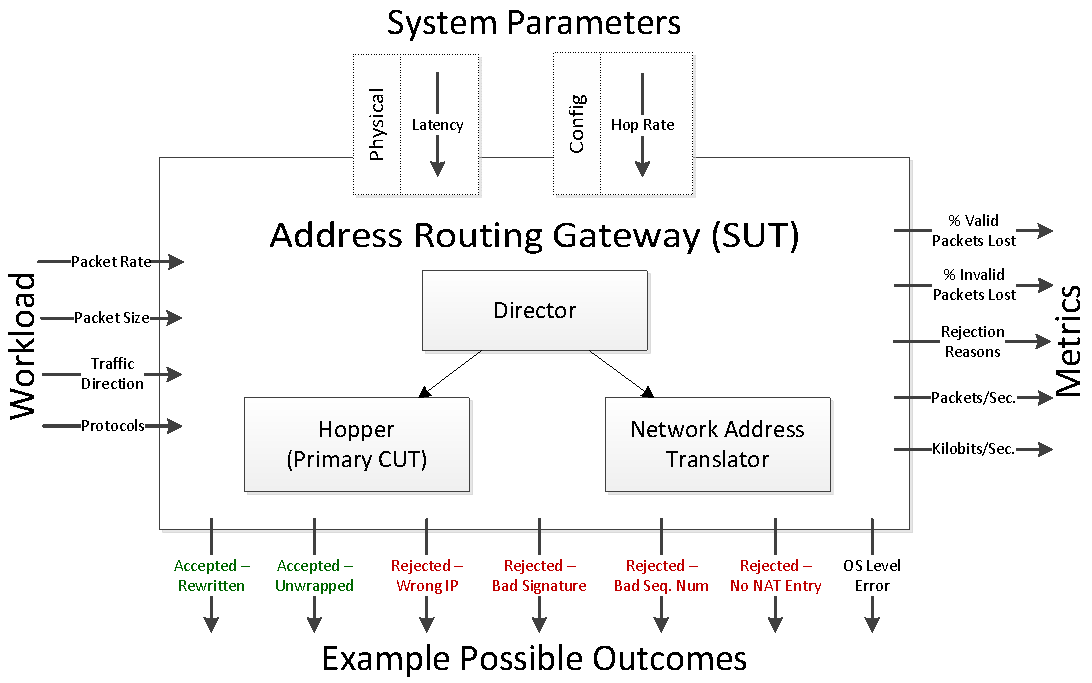
\includegraphics[width=1.2\textwidth]{sut}
}
\end{figure}

\FloatBarrier
\section{System Services}
\label{sec:services}
\par This thesis tests three components of \ac{ARG}. Most important is the hopper module, which provides a rapidly-changing external \ac{IP} address and details on connected ARG networks. Using this information, it transports packets between ARG-protected networks. Packets to and from external hosts---hosts that are not part of an ARG network---go through the \ac{NAT} module. Finally, the director module hands packets off to each of the other modules and collects the results back to be logged and potentially acted upon. More details on these components are in Chapter \ref{chp:implementation}.

\par The potential outcomes of the director are shown below, broken into separate sections based on incoming or outgoing packets. Other services do not directly offer outcomes relevant to this research.

\begin{itemize}
\item Director - Incoming
	\begin{itemize}
	\item Rewritten and forwarded - Packet is from non-\ac{ARG} network and is rewritten via \ac{NAT} table before forwarding.
	\item Unwrapped and forwarded - Packet is from \ac{ARG} network and passes validation checks. Contents are extracted and forwarded internally.

	\item Incorrect source \ac{IP} - Packet is coming from an \ac{ARG} network but does not have the what the local gateway believes is the current source IP for the other gateway.
	\item Incorrect destination \ac{IP} - Packet is coming from an \ac{ARG} network but does not have the current local gateway \ac{IP} as the destination.
	\item Incorrect message size - The message length does not match the message type.
	\item Incorrect sequence number - The message's sequence number is not monotonically increasing. 
	\item Unable to verify signature/\ac{HMAC} - Packet signature invalid/nonexistent (if coming from an \ac{ARG} network).
	\item No \ac{NAT} bucket/entry - Packet is coming from a non-\ac{ARG} network but does not have a valid entry in the \ac{NAT} table.

	\item Misc - Some operating system-level errors may occur, resulting in rare errors in sending or receiving packets.
	\end{itemize}

\item Director - Outgoing
	\begin{itemize}
	\item Rewritten and forwarded - Packet is destined for non-\ac{ARG} network. An entry is made/retrieved from the \ac{NAT} table and used to rewrite packet.

	\item Gateway not connected - Packet was intended for an ARG network the gateway is aware of but not yet connected to.
	\item Wrapped and forwarded - Packet is destined for an \ac{ARG} network. Wrapped and placed on the external network.

	\item Misc - Some operating system-level errors may occur, resulting in rare errors in sending or receiving packets.
	\end{itemize}
\end{itemize}

\section{Workload}
\label{sec:workload}
\par Workload to the system is the traffic flowing through the \ac{ARG} gateways. Standard network traffic parameters like packet rate, packet size, number of simultaneous ongoing connections, and lifetime of connections play a role. However, it is important to note that the network performance itself is not a large concern of this research. Packet rate, for example, does provide useful information about the performance of \ac{ARG} itself, but the numbers apply only to this specific implementation. \ac{ARG}'s development does not focus on performance in this first iteration, so there are many possible areas for improvement. Previous research has shown that similar solutions have minimal impact on performance \cite{NAH}. 

\par Two parameters are more specific to \ac{ARG}. First, the proportion of traffic between protected networks verses traffic to external hosts varies the validation methods \ac{ARG} uses for each packet. Traffic flows that focus on connections between protected networks rely on current \ac{IP} synchronization and signatures, while traffic that originates externally exercises the \ac{NAT} table.

\par Second, the proportion of valid and invalid traffic---traffic that should or should not be permitted through \ac{ARG}---is a workload parameter. The reasons behind each packet's invalidity is also important: most of the possible outcomes from \ac{ARG} depend on \textit{why} a packet is invalid. The possible failure points here are incorrect external \acp{IP}, invalid packet signatures, and no entry in the \ac{NAT} table.

\section{Performance Metrics}
\label{sec:metrics}
\par As previously stated, this research primarily focuses on the classification accuracy of \ac{ARG} and the interaction of hop rate and latency. Measurements on \ac{ARG} therefore concentrate on the outcomes from the director. However, basic statistics on network performance are collected. The metrics of interest include:

\begin{itemize}
\item Percentage of invalid packets accepted
	\par If a packet that should have been rejected is accepted by \ac{ARG}, it is possible for an attacker to sneak into the network regardless of the gateway's existence. This is the true measure of whether or not \ac{ARG} is protecting the network. If \ac{ARG} functions correctly, this number should remain at zero for all experiments with \ac{ARG} enabled.

\item Percentage of valid packets rejected
	\par In ideal circumstances, this will also be zero. However, network conditions may result in failures here, which on a real-world network might result in a disruption of service. 

\item Number of each type of rejection (each possible outcome from the director)
	\par This reveals where in the processing stage packets are typically caught. If packets get caught in the later stages of validation---e.g., signature checking---then processing time has been wasted.

\item Packets per second and \acf{Kbps}
	\par An easy check on \ac{ARG}'s performance is comparing the amount of traffic it is handling against the packet loss it shows. Information about both the number of packets and the raw number of bits it processes may reveal slightly different results, so both are collected.
\end{itemize}

\section{System Parameters}
\label{sec:parameters}
\par As a network application, \ac{ARG} is affected by both the machine on which it runs and the network over which it communicates. \ac{ARG}'s local performance is most affected by processor and memory speeds, with encryption potentially consuming a fair amount of processor time and memory speeds impacting virtually all aspects of operation.

\par The primary physical network parameter that affects \ac{ARG} is latency. To ensure that two \ac{ARG} gateways are able to communicate reliably, packets sent from one gateway to the other must arrive before the \ac{IP} addresses used in the send are no longer current. If hops occur too frequently, then a high one-way latency will cause sent packets to frequently arrive after the receiving gateway has hopped to a different \ac{IP} address. 

\par The primary configuration setting for \ac{ARG} is the hop rate. \ac{ARG} allows the time between hops to be customized from several times a second to minutes apart with millisecond precision. Each gateway may be configured to hop at different rates, but for the sake of this thesis the hop rates are always identical in a given test.

\section{Factors}
\FloatBarrier
\label{sec:factors}
\par Based on the system and workload parameters given above, the following factors are varied as part of the experiment. All others remain constant throughout the experiment. Factors and levels are summarized in Table \ref{tbl:factors} and described in detail below.

\begin{table}
\begin{center}
	\caption{Experimental factors and levels}
	\label{tbl:factors}
	
	\begin{tabular}{r|l}
	\textbf{Factor} & \textbf{Possible Levels} \\
	\hline
	Hop rate (ms) & 1000, 500, 300, 200, 100, 75, 60, 50, 40, 30, 15, 10, 5\\
	Round-trip latency (ms) & 500, 100, 30, 20, 0\\
	Packet delay (s) & 0.3, 0.2, 0.1, 0.05, 0.01, 0.005, 0.001\\
	Traffic direction and type & See detailed description
	\end{tabular}
\end{center}
\end{table}

\begin{itemize}
\item Hop rate
	\par Varying the rate at which \ac{ARG} switches to a new external \ac{IP} allows testing of the maximum supportable hop rate. Hops every 1000 milliseconds give ample time for packets to travel across the network at all but the most extreme latencies, while hops every 5 milliseconds stress even ideal network conditions.

\item Latency between \ac{ARG} gateways
	\par The test network runs through a single switch running four \acp{VLAN}, with an average latency under 1 millisecond. Introducing artificial latency simulates a more realistic range of environments.

\item Packet Delay
	\par Each test spawns a number of traffic generators at different points in the test network. The packet delay shown here is used as a wait between each packet sent. Lower delays result in more frequent sends and force the gateways to deal with more packets per second.

\item Traffic direction and type
	\par \ac{ARG} is capable of handling \ac{TCP}, \ac{UDP}, and \ac{ICMP} traffic. All tests use equal amounts of \ac{TCP} and \ac{UDP} traffic, but some vary the direction. Section \ref{sec:exp_design} gives a full description of the various tests and Figure \ref{fig:testnum_flows} illustrates the direction of all traffic on the network.
\end{itemize}

\section{Evaluation Technique}
\label{sec:eval_technique}
\par Measurement is used to obtain results for each factor level. Due to the fairly complex interactions needed between \ac{ARG} gateways and the processing needed to decide how to handle packets, simulating the system would likely require an equal amount of work with little benefit.

\par Setup of the test environment involves a basic 7-node network: three gateways running \ac{ARG}, one system on the network protected by each gateway, and one host outside the network. Figure \ref{fig:argnetwork} shows the network and the names given to the various systems.

\begin{figure}
	\centering
	\caption{\ac{ARG} test network layout overview}
	\label{fig:argnetwork}
	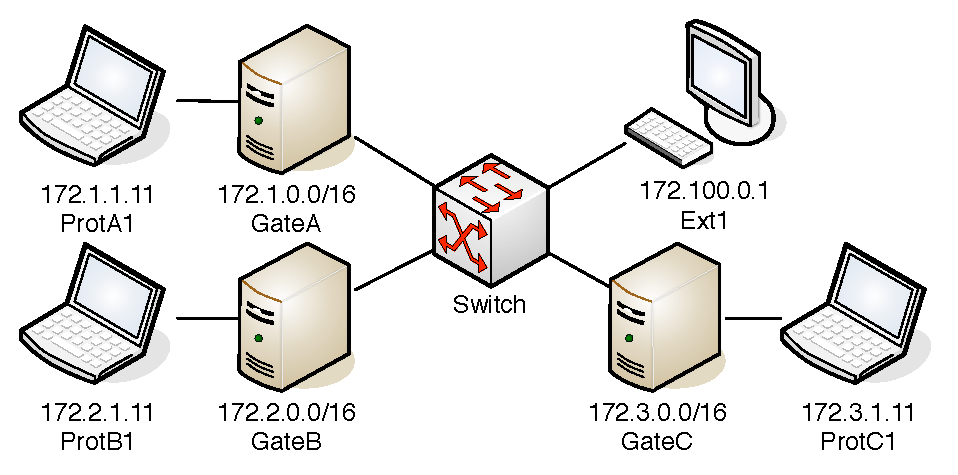
\includegraphics[width=0.75\textwidth]{thesis_network}
\end{figure}

\par Protected clients behind the gateways (\texttt{ProtA1}, \texttt{ProtB1}, and \texttt{ProtC1}) may communicate freely. The protected clients may also talk out to the external host (\texttt{Ext1}), and the external hosts must then---once that connection is established---be able to talk back into the network. There is additional administrative traffic directly between the gateways (\texttt{GateA}, \texttt{GateB}, and \texttt{GateC}). These three basic traffic flows are ``valid'' traffic.

\par All traffic beyond what is described above is ``invalid.'' For example, \texttt{Ext1} is not allowed to send traffic in to the protected clients or the gateways without them first initiating the connection. Malformed traffic sent by any host is also considered invalid. In either case, invalid traffic should be stopped at the earliest possible opportunity (i.e., the gateway rejects the packet and keeps it from reaching the internal host) and the gateway must remain stable.

\par To collect data, each system runs the traffic collection program \texttt{tcpdump} to capture the traffic sent and received into \ac{PCAP} files. Traffic generators are then spawned as appropriate on each system in the network, each of which logs their sends and receives. After a given trial, the \ac{PCAP} files and traffic generator logs are collated and processed with custom scripts to determine the metrics described in Section \ref{sec:metrics}. More details on the traffic generators and test run sequence can be found in Appendixes \ref{chp:testseq} and \ref{chp:generators}. Appendix \ref{chp:processor} covers the custom results processor.

\par All trials run on network of seven physical servers. Each server runs Ubuntu 12.04.1 Server Edition with four gigabytes of \ac{RAM} and a 2.6 gigahertz quad-core Intel Xeon. A single switch with four \acp{VLAN} connects each system at 100 \ac{Mbps}.

\section{Experimental Design}
\label{sec:exp_design}
\par Based on the factors given in Section \ref{sec:factors} and the goals of this research (as Section \ref{sec:goals} lays out), there are eight traffic flows of interest. Each consists of different types of traffic and flow destinations. These are most easily visualized in Figure \ref{fig:testnum_flows}.

\begin{figure}
\caption[Experiment traffic flow directions and protocols]{Experiment traffic flow directions and protocols. Black is valid traffic, red is invalid.}
\label{fig:testnum_flows}
\centering
\begin{subfigure}[b]{0.328\linewidth}
	\centering
	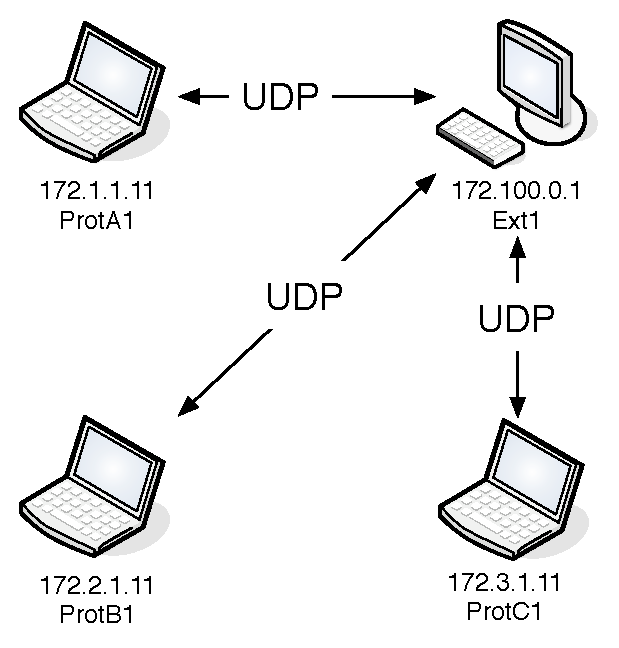
\includegraphics[width=1.0\linewidth]{test_traffic_0}
	\caption{Test 0}
\end{subfigure}
\begin{subfigure}[b]{0.328\linewidth}
	\centering
	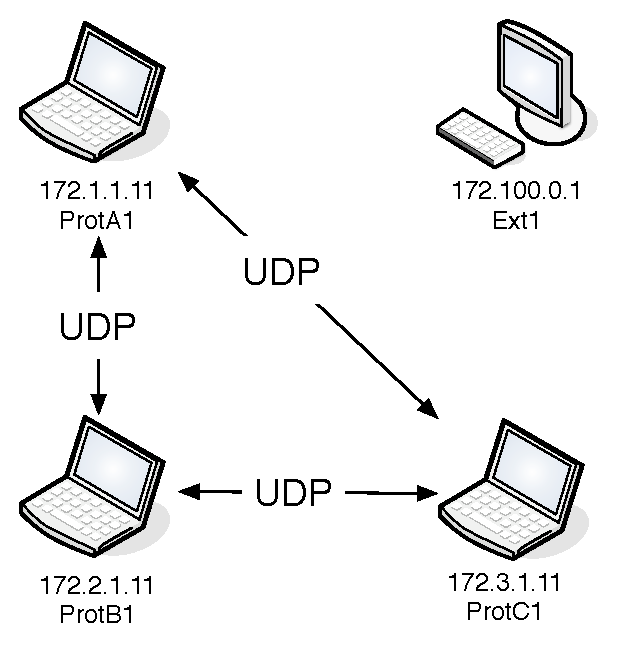
\includegraphics[width=1.0\linewidth]{test_traffic_1}
	\caption{Test 1}
\end{subfigure}
\begin{subfigure}[b]{0.328\linewidth}
	\centering
	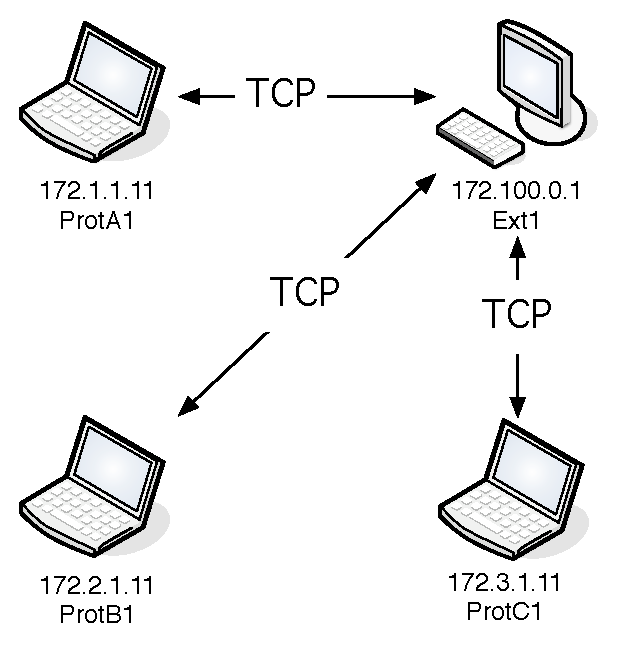
\includegraphics[width=1.0\linewidth]{test_traffic_2}
	\caption{Test 2}
\end{subfigure}
\begin{subfigure}[b]{0.328\linewidth}
	\centering
	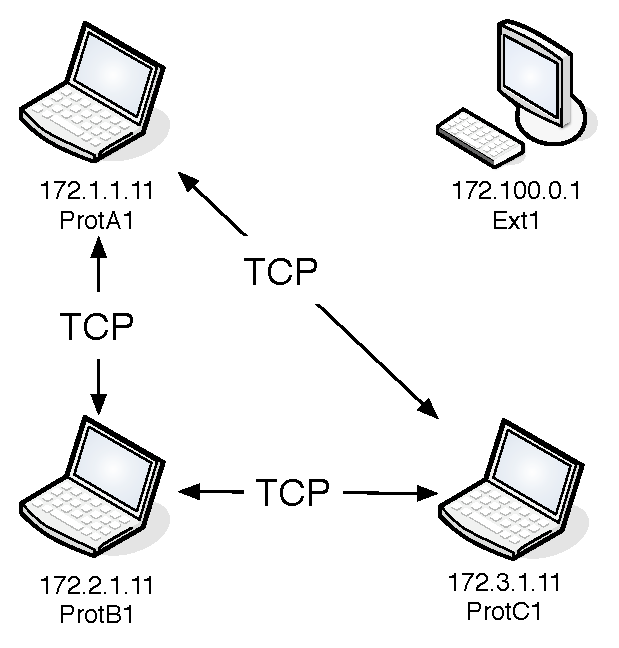
\includegraphics[width=1.0\linewidth]{test_traffic_3}
	\caption{Test 3}
\end{subfigure}
\begin{subfigure}[b]{0.328\linewidth}
	\centering
	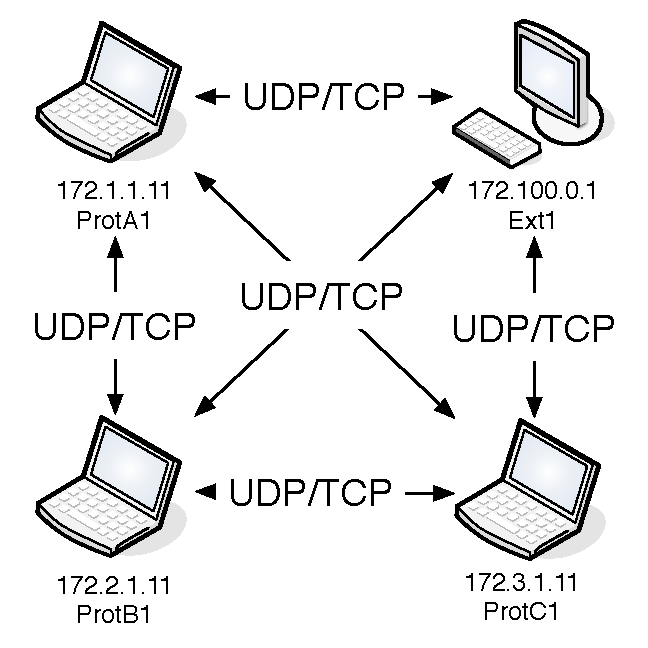
\includegraphics[width=1.0\linewidth]{test_traffic_4}
	\caption{Test 4}
\end{subfigure}
\begin{subfigure}[b]{0.328\linewidth}
	\centering
	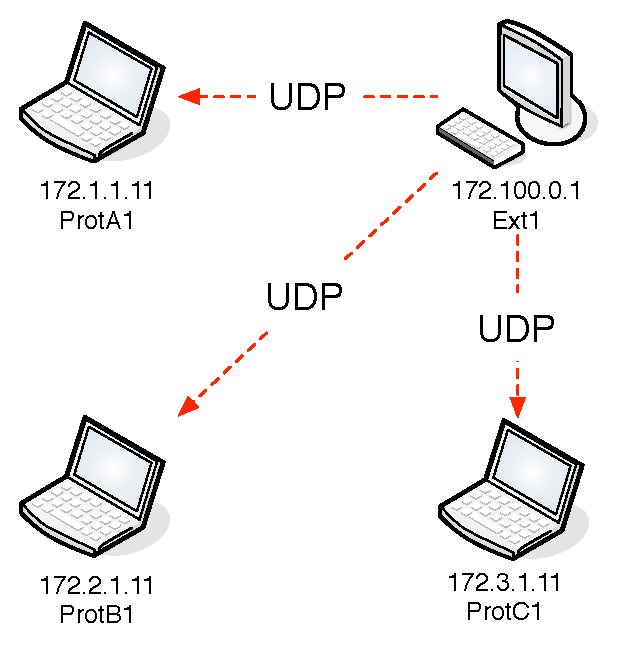
\includegraphics[width=1.0\linewidth]{test_traffic_5}
	\caption{Test 5}
\end{subfigure}
\begin{subfigure}[b]{0.328\linewidth}
	\centering
	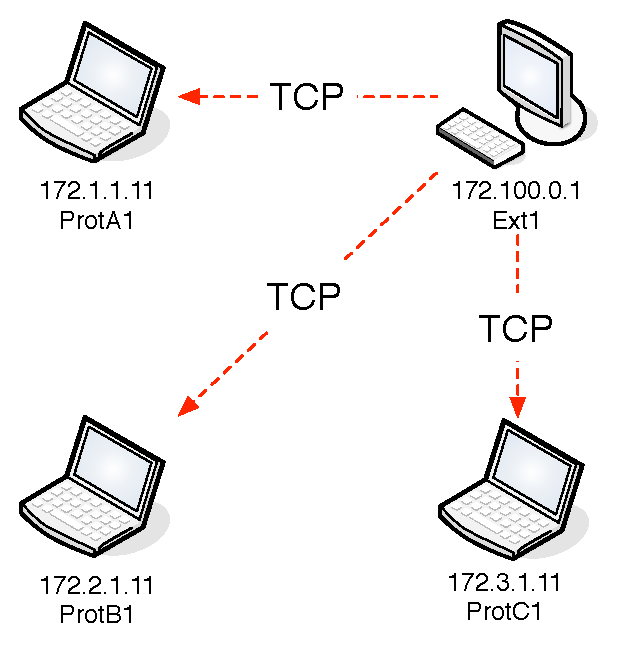
\includegraphics[width=1.0\linewidth]{test_traffic_6}
	\caption{Test 6}
\end{subfigure}
\begin{subfigure}[b]{0.328\linewidth}
	\centering
	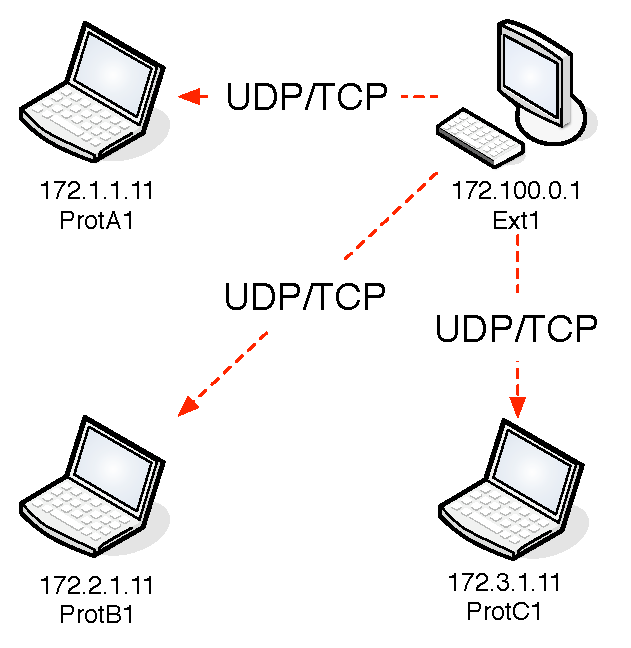
\includegraphics[width=1.0\linewidth]{test_traffic_7}
	\caption{Test 7}
\end{subfigure}
\begin{subfigure}[b]{0.328\linewidth}
	\centering
	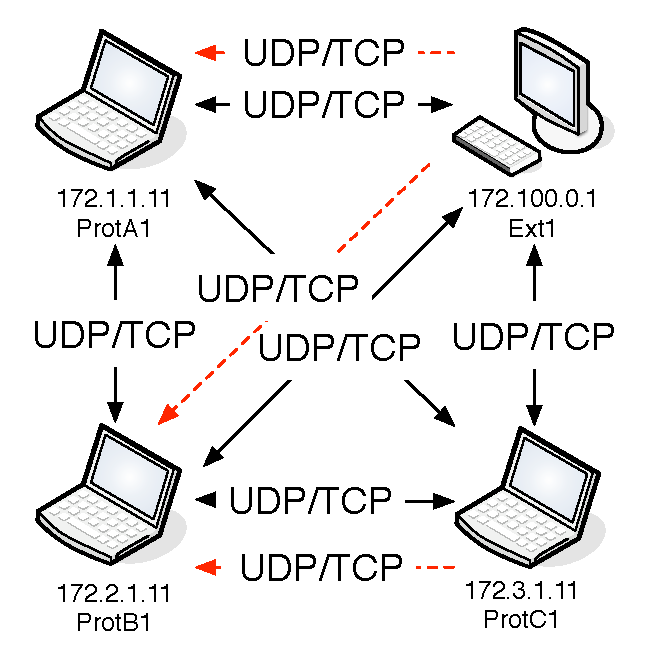
\includegraphics[width=1.0\linewidth]{test_traffic_8}
	\caption{Test 8}
\end{subfigure}
\end{figure}

\par These possible traffic flows are used in four sets of experiments, given below. Each experiment set answers a different research goal.
\begin{itemize}
	\item Basic tests
	\par This sequence of tests verifies that \ac{ARG} classifies traffic correctly by running every test shown in Figure \ref{fig:testnum_flows} against \ac{ARG}. Latency is set to 20 milliseconds (\ac{RTT}) for all tests and traffic generators produce packets around every 0.3 seconds (actual traffic rate is higher due to responses and \ac{TCP} acknowledgment packets). To determine if hop rate has an large impact on certain types of traffic, every test runs twice, once with a slow hop rate (500 ms) and one close to double the latency (50 ms).

	\item Max Throughput
	\par This sequence gives an indication of what throughput and packet rate \ac{ARG} is capable of handling. Packet delay goes through all levels shown in Table \ref{tbl:factors}, which leads to roughly corresponding increases in the throughput the gateways must handle. Hop rate changes between 500 ms and 50 ms to see if the additional \ac{IP} calculation load impacts the maximum rate. Test 4 is used in all runs to exercise all possible valid traffic flows. \ac{RTT} is set to 20 ms.

	\item Max hop rate
	\par This sequence determines the maximum hop rate at various latencies. Hop rate and latency go through the levels shown in Table \ref{tbl:factors} in a full factorial fashion (every latency-hop rate combination). Packet rate is fixed at 0.3 seconds and Test 4 is used throughout.

	\item Fuzzer
	\par This sequence is not tested rigorously for traffic flow success and failure, but ensures that \ac{ARG} remains stable despite malformed traffic. Test 8 is used, with the addition of fuzzers on each gateway that replay and/or alter traffic they see. Hop rate varies between 500 ms and 50 ms, latency is fixed at 20 ms, and packets are sent at 0.3 second intervals.
\end{itemize}

\par A 95\% confidence interval is used for all experiments. Experiments are each run for five minutes, sufficient time for the system to stabilize (pilot studies show that \ac{ARG} fully connects in under 10 seconds on the test network). Wide variation is possible in the actual traffic seen in a single run, so a minimum of 10 replications are used for each experiment.

\section{Summary}
\label{sec:method_summary}
\par This chapter discusses the goals of this research and defines the \ac{SUT} and its relevant factors. The methodology in use is covered, with details on the test network and the exact tests run on this network. Finally, this chapter enumerates the metrics the tests collect and analyze. 


\lettrine{T}{here} are two distinct parts here:

\par Conclusions: Re-state what you have done, summarize the results that you got,
and summarize the key conclusions that you can draw from your results. All of
this is a summary of the entire thesis, and there should be absolutely nothing new
here that hasn’t already been covered in the previous chapters. (It will probably
be presented in a more concise form, however—don’t just cut-and-paste from
previous chapters).

\par Recommendations: Think of this as a description of what should be done in any
follow-on work (as if a student is picking up where you left off, and you need to
tell them what they could/should look at). I’ve found that a bulleted list of
recommendations often works well, where each bullet is a paragraph (or two)
describing a particular recommendation that you have. Don’t be afraid to point
out the shortcomings of your work, and describe what would need to be done to
overcome these shortcomings. (Doing so shows that you understand the limits of
your research, and comes off far better than trying to pretend that your research
has solved every problem, when it really hasn’t). Much of what is covered here
will have already been stated in the analysis of Chapter 4. However, it’s OK to
have some new concepts here that aren’t explicitly described elsewhere.

\par As networks are hit harder each day by increasingly sophisticated attackers, new methods of defending the the systems inside must be developed. An active measure such as IP address hopping has been shown to provide additional protection from network enumeration \cite{NAH}, traffic sniffing \cite{BBNDYNAT}, and exploitation \cite{APOD}.

\par The Address Routing Gateway this paper proposes accomplishes these goals through master gateways that transform traffic without any changes needed to the networks they protect. Previous systems tend to either have a more limited protection scope or require broader changes to existing equipment and networks. While a prototype needs to be implemented to fully demonstrate the system's capabilities, previous work indicates that the overhead associated with the introduced of ARG would fall into an acceptable range \cite{NAH}.

\par Finally, it is hoped that ARG can be linked with a honeypot and/or intrusion detection system. ARG's unique ability to detect unexpected, potentially malicious packets makes it possible to track the actions of an adversary's actions. This may reveal the identity of an adversary, their goals, and their intended target in the network, all valuable information to those defending the network.


\chapter{Conclusions and Recommendations}
\label{chp:conclusion}
\par This chapter summarizes the work and findings of this research. Section \ref{sec:research_conclusions} summarizes the conclusions reached in this research. Section \ref{sec:research_impact} discusses the impact of this research. Section \ref{sec:future_work} provides recommendations for future work in this area.

\par As networks are hit harder each day by increasingly sophisticated attackers, new methods of defending the the systems inside must be developed. An active measure such as IP address hopping has been shown to provide additional protection from network enumeration \cite{NAH}, traffic sniffing \cite{BBNDYNAT}, and exploitation \cite{APOD}.

\par The Address Routing Gateway this paper proposes accomplishes these goals through master gateways that transform traffic without any changes needed to the networks they protect. Previous systems tend to either have a more limited protection scope or require broader changes to existing equipment and networks. While a prototype needs to be implemented to fully demonstrate the system's capabilities, previous work indicates that the overhead associated with the introduced of ARG would fall into an acceptable range \cite{NAH}.

\section{Research Conclusions}
\label{sec:research_conclusions}
\par This research has found that \ac{IP} hopping is a suitable method of blocking unexpected external traffic while having a minimal false-positive rate. This can be done in a way completely transparent to the internal and external hosts; the tool developed here works with no configuration changes to other hosts.

\par In addition, \ac{ARG} proves rapid \ac{IP} changes are possible, with network latency as the primary limiter. \ac{ARG} also demonstrates solid throughput, a critical aspect of deployability to a real network.
\tbd{fuzzer}

\section{Research Impact}
\label{sec:research_impact}
\tbd{sample has this... not in document}

\section{Future Work}
\label{sec:future_work}
\subsection{IPv6 support}
\par \ac{IPv6} support is slowly becoming an absolute requirement for any network system. For a \ac{IP} hopping system, \ac{IPv6} offers the benefit of a greatly increased address space, allowing systems to hop in a much broader range of addresses. \ac{ARG} is entirely \ac{IPv4} in its operation and cannot transport \ac{IPv6} packets to external hosts or to other gateways.

\subsection{Fragmentation Support}
\par \tbd{tbd}

\subsection{More extensive malicous testing}
\par Due to time constraints, a full battery of robust malicious tests could not be performed against \ac{ARG}. As demonstrated by the basic fuzz testing, \ac{ARG} handles errors without dying, but may lose additional packets. The reasons behind this potential issue needs more exploration to determine the root cause and what should be done to fix it. More extensive work in both undirected (i.e., fuzz testing) and directed attacks is needed. For example, malicious hosts might attempt to falsly connect to a gateway or perform replay attacks in a more intelligent manner.  

%\subsection{Red teaming}
%\par In conjunction with the previous suggestion, 

\subsection{More intelligent NAT}
\par \ac{ARG} currently blindly opens holes in the \ac{NAT} when it sees outbound packets and closes them after seeing no activity in a fixed amount of time. A transport layer examination would allow more fine-grained \ac{NAT} work, by watching for actual connection establishment and teardown packets. 

\subsection{Integration with other defenses}
\par Network defenses often perform better when working in tandem. \ac{ARG} has the potential to detect certain types of probes into the network. If this information could be passed off to an \ac{IDS}, it might alert an operator or take other defense actions on the network. In an even more active approach, \ac{ARG} might work with a honeypot to present a fake view of the network to an attacker. By examing what systems an attacker probes, it might be possible to determine the identity of the adversary, their goals, and their intended target in the network, all valuable information to those defending the network.

\section{Summary}
\par This chapter reviews the work and findings of this thesis. The impact of the research is discussed and recommendations for future work are given.



%%%%%%%%%%%%%%%%%%%%%%%%%%
% Appendices
%%%%%%%%%%%%%%%%%%%%%%%%%%
\appendix
\begin{landscape}
\chapter{\ac{IP} Packet Structure}
\label{chp:ip_packet}
\begin{table}
\caption{\ac{IP} packet structure}
\label{tbl:packet_structure}
\centering
\includegraphics[clip,trim=.3in 5in 0 0]{packet_structure}
\end{table}
\end{landscape}


\chapter{\ac{ARG} Protocol}
\label{chp:protocol}
\par This appendix details the format of each \ac{ARG} message type. Section \ref{sec:arg_protocol_formats} presents the structure of each message type. Section \ref{sec:arg_protocol_exchanges} gives the steps of each exchange type and their effect on the gateway's state.

\section{Message Formats}
\label{sec:arg_protocol_formats}
\par The base header for the \ac{ARG} protocol is given in Table \ref{tbl:arg_protocol_types}. Four possible payloads are delivered under this header: \texttt{WRAPPED}, \texttt{PING}, \texttt{CONN\_REQ}/\texttt{CONN\_RESP}, and \texttt{TRUST\_DATA}. The format for each is shown in individual sections below.

\subsection{\texttt{WRAPPED}}
\par Use: Transfer packets between \ac{ARG}-protected networks.

\par This message type contains no additional information. After the original packet is encrypted, it is used as the payload to the \ac{ARG} header as-is.

\subsection{\texttt{PING}}
\par Use: Time synchronization between two gateways. See Section \ref{sec:arg_time_sync}.

\begin{table}[H]
\caption{Data in \ac{ARG} \texttt{PING} message}
\label{tbl:arg_ping_struct}
\centering
\begin{tabular}{l|l|l}
\textbf{Data} & \textbf{Size} & \textbf{Data Type}\\
\hline
Request ID & 4 bytes & Integer\\
Response ID & 4 bytes & Integer\\
Time Offset & 4 bytes & Integer
\end{tabular}
\end{table}

\subsection{\texttt{CONN\_REQ}/\texttt{CONN\_RESP}}
\par Use: Connect to other gateways.

\par Note that these message types are formatted identically. The only difference is the type number used, as this allows gateways to determine when it is a request for new data or just a response to a previous request.

\begin{table}[H]
\caption{Data in \ac{ARG} \texttt{CONN\_REQ} and \texttt{CONN\_RESP} messages}
\label{tbl:arg_conn_data_struct}
\centering
\begin{tabular}{l|l|l}
\textbf{Data} & \textbf{Size} & \textbf{Data Type}\\
\hline
Symmetric Key & 32 bytes & Raw\\
\ac{IV} & 32 bytes & Raw\\
Hop Key & 16 bytes & Raw\\
Hop Interval & 4 bytes & Integer
\end{tabular}
\end{table}

\subsection{\texttt{TRUST\_DATA}}
\par Use: Allow on-the-fly addition of new gateways.

\begin{table}[H]
\caption{Data in \ac{ARG} \texttt{TRUST\_DATA} message, 4 bytes wide}
\label{tbl:arg_trust_struct}
\centering
\begin{tabular}{l|l|l}
\textbf{Data} & \textbf{Size} & \textbf{Data Type}\\
\hline
Gate Name & 10 bytes & Null-padded String\\
Base \ac{IP} & 4 bytes & Integer\\
Mask & 4 bytes & Integer\\
N & 130 bytes & Raw\\
E & 10 bytes & Raw
\end{tabular}
\end{table}

\section{Protocol Exchanges}
\label{sec:arg_protocol_exchanges}
\par The steps for each exchange are given in the sections below. In the following descriptions, local is the initiating gateway in a given exchange and remote is another gateway with which it is communicating.

\subsection{Connect process}
\begin{enumerate}
	\item Local sends \texttt{CONN\_REQ} containing its hop key, hop interval, and symmetric key. 
	\item After validating the packet, remote saves the connection data. If time synchronization data is available for local, then remote marks it as connected. If it is not available, remote schedules a time synchronization request.
	\item Remote sends \texttt{CONN\_RESP} acknowledgment back, containing its own hop key, hop interval, and symmetric key. 
	\item Local receives, validates, and saves the data from remote.
	\item Local marks the remote gateway as having connection data and marks remote as connected or schedules a time sync, as appropriate.
\end{enumerate}

\subsection{Time synchronization}
\label{sec:arg_time_sync}
\begin{enumerate}
	\item Local sends \texttt{PING} containing random 4-byte unsigned integer in the \texttt{Request ID} field (see Table \ref{tbl:arg_ping_struct}), \texttt{null} (0) in \texttt{Response ID}, and its time offset in \texttt{Time Offset}, which is the different between the current time and its base time. 
	\item Local notes the time it sent the request
	\item Remote validates the message and responds with a new \texttt{PING}, giving a new random request integer, the received response int (from local) set to the request int, and its own time offset.
	\item Local ensures received response int matches the request int it sent.
	\item Local determines the connection latency from the send time, then remote's time base is calculated based on half of this. That is,
	$$\text{remote time base} = \text{received time offset} - \frac{\text{latency}}{2}$$
	This value is saved and used in \ac{IP} calculations for the remote gateway in the future.

	\item Local marks the remote gateway as having time sync data available and, if connection data is available, remote is marked as connected. If connection data is not available, local schedules a connect process.
	\item Local sends a response to remote, with \texttt{Request ID} set to 0, \texttt{Response ID} set to the value remote sent in its request, and time offset set as appropriate.
	\item Remote receives and validates the final response, saves off the data, and marks local as connected if appropriate (or schedules a connection data request if needed).
\end{enumerate}

\subsection{Trust Data Exchange}
\begin{enumerate}
	\item For each gateway it knows about, local sends a \texttt{TRUST\_DATA} packet to remote, containing the gateway name, base \ac{IP}, \ac{IP} mask, and public key to the remote gateway. Each packet covers one gateway, with no data about the local or remote gateways included.
	\item Remote validates the message, then adds the data in each \texttt{TRUST\_DATA} packet to their list of gateways (if they don't already have it). At this point the new gateway appears just like one read in from a configuration file.
	\item After some period of time, remote attempts to connect to the new gateway, just as they would any other gateway they had not yet successfully contacted.
 \end{enumerate}

\subsection{Route packet}
\label{sec:arg_protocol_route}
\begin{enumerate}
	\item Local receives a packet on its internal interface.
	\item Local takes the outbound packet and encrypts with with remote symmetric key. Local determines the destination gateway based on \ac{IP} range.
	\item Local sends WRAPPED message to remote current IP with the encrypted packet included. An \ac{HMAC} of the packet (encrypted data and headers) is included in the header.
	\item Remote receives and validates the message.
	\item Remote sends the original, decrypted packet into the internal network.
\end{enumerate}


\chapter{\ac{ARG} Testing}
\label{chp:testseq}
\par This appendix covers the precise setup of the test environment and the steps used to run a test. 

\section{Network Setup}
\par 

\section{Test Sequence}
\par For each test, the events shown below occur, in order. The script that executes them includes additional safety measures, such as ensuring none of the components are already running (and killing them if they are), but these are not included.

\singlespace{
\begin{enumerate}
\item Set time on all hosts to be the as similar as possible (used for post-processing only).
\item Set artificial network latency on external interfaces of gates.
\item Start \texttt{tcpdump} on each host. Gateways have two instances started, one for each interface. \tbd{tcpdump filters?}
\item Set \ac{ARP} cache size on gateways and external host to allow for 65536 entries. This is needed at high hop rates only because everything is on the same network segment.
\item Push configuration files for \ac{ARG}. \texttt{ProtA1} and \texttt{ProtC1} each know about \texttt{ProtB1}, but not about each other. \texttt{ProtB1} knows about both.
\item Start \ac{ARG} on the gateways. 
\item Start traffic generators on hosts, as appropriate for the test being run. See Section \ref{sec:exp_design} for general flow of traffic for each test type.
\item Wait for however long is needed for the test. For all tests discussed in this thesis, tests run for five minutes.
\item Stop traffic generators.
\item Stop \ac{ARG}.
\item Stop traffic collectors (\texttt{tcpdump}).
\item Retreive log and pcap files from every host into a directory.
\end{enumerate}
}

\par After the logs are collected together, the run is processed by a separate script, \texttt{process\_run.py}. See Appendix \ref{chp:processor} for details on its use. 


\chapter{\ac{ARG} Building and Configuration}
\label{chp:argconf}

\par This appendix documents everthing needed to use \ac{ARG}. Section \ref{sec:arg_env} covers the build environment needed to build \ac{ARG} from source. Section \ref{sec:arg_cmd} documents calling \ac{ARG} and creating the necessary configuration files.

\section{Building}
\label{sec:arg_env}
\par \ac{ARG} runs on Ubuntu 12.04 and 12.10. Other versions and distributions are untested, although they may work if the below requirements are met. 

\subsection{Required Packages}
\tbd{versions}
{\singlespace
\begin{itemize}
\item gcc $>=$4
\item linux-headers
\item Autoconf $>=$2.69
\item Automake
\item libtool
\item libpcap-dev
\item librt-dev
\item libpthread-dev
\item libpolarssl-dev
\end{itemize}
}

\par In Ubuntu:
\begin{lstlisting}[language=bash]
sudo apt-get install automake autoconf build-essential libtool libpcap-dev libpolarssl-dev
\end{lstlisting}

\subsection{Compilation}
\par From the \ac{ARG} source directory:
\begin{lstlisting}[language=bash]
./autogen.sh
make
\end{lstlisting}

\par This should produce two executables, \texttt{arg} and \texttt{gen\_gate\_config}.

\section{Running}
\label{sec:arg_cmd}
\subsection{Synopsis}
\par \ac{ARG} must be run 


\chapter{Traffic Generators}
\label{chp:generators}


\chapter{Results Processor}
\label{chp:processor}

\par After every test run, a custom utility processes the pcap and log files into a single database and extracts statistics from there. This appendix documents the usage of this tool and its operation. Section \ref{sec:proc_env} covers the required packages to process runs. Section \ref{sec:proc_usage} covers usage of the results processor. Section \ref{sec:proc_operation} documents the operation of the processor.

\section{Validation}
\par Validation is done manually on this tool via short, extremely low-traffic test runs. By performing tests with only a few packets in each direction, it is possible to manually ensure that all results the processor produces are accurate. These validation tests are done on everything from single-flow tests (one direction between just two hosts) and many-flow, multi-protocol tests.

\section{Environment}
\label{sec:proc_env}
\par The test processor runs on Ubuntu 12.04, Ubuntu 12.10, and Mac OSX 10.8. Other versions and distributions are untested, although they may work if the below requirements are met. 

\par The following packages must be available for \texttt{process\_run.py} to run:

{\singlespace
\begin{itemize}
\item Python 2.7
\item python-scapy $>=$2.2.0
\item python-libpcap $>=$0.6.2
\end{itemize}
}

\par In Ubuntu:
\begin{lstlisting}[language=bash]
sudo apt-get install python-libpcap python-scapy
\end{lstlisting}

\section{Usage}
\label{sec:proc_usage}
\par \texttt{process\_run.py} supports a variety of parameters, all of which are optional. The full parameter list and defaults are given in Table \ref{tbl:process_run_param}. Full descriptions of each are given in the list below.

\begin{table}
\caption{\texttt{process\_run.py} command-line parameters}
\label{tbl:process_run_param}
\centering
\begin{tabular}{lll}
\toprule
\textbf{Parameter} & \textbf{Short} & \textbf{Default}\\
\hline
\texttt{--help} & \texttt{-h} & \\
\texttt{--logdir} & \texttt{-l} & `.' \\
\texttt{--database} & \texttt{-db} & In-memory\\
\texttt{--empty-database} & & false\\
\texttt{--skip-processing} & & false\\
\texttt{--skip-stats} & & false\\
\texttt{--offset} & & 0\\
\texttt{--start-offset} & & 0\\
\texttt{--end-offset} & & 0\\
\texttt{--show-cycles} & & false\\
\texttt{--finish-indicator} & & none\\
\bottomrule
\end{tabular}
\end{table}

\begin{itemize}
\item \texttt{--help} - Display usage message.
\item \texttt{--logdir}, \texttt{-l} - Path of directory with log and pcap files.
\item \texttt{--database}, \texttt{-db} - Path to database of processed run data. Will be created if needed, otherwise existing data will be used. If the database is only partially processed, \texttt{process\_run.py} will complete it. If not given, defaults to an entirely in-memory database.
\item \texttt{--empty-database} - If given, all existing data in database is removed.
\item \texttt{--skip-processing} - Do not attempt to process data, only produce results. If the database is incomplete, nothing will happen.
\item \texttt{--skip-stats} - Do not calculate statistics after processing run data.
\item \texttt{--offset} - Number of seconds to ignore at the beginning and end of a run.
\item \texttt{--start-offset} - Number of seconds to ignore at beginning of run. Overrides value of \texttt{--offset}.
\item \texttt{--end-offset} - Number of seconds to ignore at end of run. Overrides value of \texttt{--offset}.
\item \texttt{--show-cycles} - If processing errors occur and the processor generates loops in the packet chains (i.e., following the next hop for each packet eventually would lead back around), show cycles may reveal the problem packet(s). Mostly obsolete.
\item \texttt{--finish-indicator} - File to create after processing is complete. Intended for automation.
\end{itemize}

\subsection{Example}
\par The most common use case, when the caller wants to process the run data in the current directory and create a database named \texttt{run.db} with the results:
\begin{lstlisting}
~/results/basic-t0-l20-hr500ms-2012-11-24-08:54:21$ process_run.py -db run.db
\end{lstlisting}

\par If a run takes several seconds to enter a steady state, it may be beneficial to ignore the first 30 seconds of the run. In addition, this example does its work from a different directory but leaves the results in the same location as the previous example:
\begin{lstlisting}
~/results$ process_run.py -l basic-t0-l20-hr500ms-2012-11-24-08:54:21 -db basic-t0-l20-hr500ms-2012-11-24-08:54:21/run.db --start-offset 30
\end{lstlisting}

\section{Processor Execution}
\label{sec:proc_operation}
\par Run processing follows the steps below. It makes assumptions about the test network to determine where packets are headed and what hosts actually send and receive them, so logs must come from a network set up as documented in Figure \ref{fig:argnetwork}.

\begin{enumerate}
\item Create database.
\item Read run settings from log files and file names.
\item Check settings for test setup problems, such as missing hosts.
\item Read through each \ac{PCAP} file, entering every packet into the database with a hash of its data.
\item Read through each log file. For each send/receive/transformation (gateways passing a packet to/from their inside network) line:
	\begin{enumerate}
	\item Determine the single-hop source and destination of the packet (who sent it and which system should see it next).
	\item Determine the true sender and receiver of packet. That is, who originally sent the packet and for whom it is intended.
	\item Determine if it is intended to be a ``valid'' packet (i.e., should it reach its destination or not?).
	\item Locate the packet in the database via hash and record the log information in the record.
	\item If it is a transformation packet (at a gateway), locate the send and receive packets and link them together.
	\end{enumerate}
\item Trace packets through the network, creating a chain of sends and receives. Packets that pass through the gateway follow the transformation through. That is, if the gateway receives a packet, alters it, and sends it out the other side, the packet sequence continues unbroken.
\item Check for packet cycles, which would indicate a tracing problem.
\item Copy true source and destination of each packet chain into all packets in the sequence. When a host sends a packet, it has an intended recipient. This information is copied into each packet in the chain, making it easier to look up.
\item Locate packet chain terminations. Each packet in a chain is given the ID number of the packet that ends the chain, allowing the processor to tell where each packet ended and if it reached the intended destination.
\item Produce statistics by querying the database for packets matching various criteria, such as packets that terminate at a different destination than intended.
\end{enumerate}



\references{
  \bibliographystyle{alpha} % or alpha, thesnum3, ieeetr, spie, aiaa, etc.
  \bibliography{research,rfc}
 }

\end{document}

